\documentclass[10pt,twocolumn,a4paper]{article}
\usepackage[utf8]{inputenc}
\usepackage[T1]{fontenc}
\usepackage{times}
\usepackage{textcomp}
\usepackage[margin=2.1cm,columnsep=0.65cm]{geometry}
\usepackage{amsmath}
\usepackage{graphicx}
\usepackage{booktabs,tabularx,array,longtable}
\usepackage{xcolor}
\usepackage{tikz}
\usepackage{adjustbox}
\usetikzlibrary{arrows.meta,positioning,shapes.symbols}
\usepackage[font=small,labelsep=colon,skip=4pt]{caption}
\usepackage{enumitem}
\usepackage{cite}
\usepackage{fancyhdr}
\usepackage[hidelinks]{hyperref}
\usepackage{xurl}
\setlist{nosep,leftmargin=*}
\DeclareUnicodeCharacter{2212}{\ensuremath{-}}
\DeclareUnicodeCharacter{2265}{\ensuremath{\geq}}
\DeclareUnicodeCharacter{2264}{\ensuremath{\leq}}
\DeclareUnicodeCharacter{00D7}{\ensuremath{\times}}
\DeclareUnicodeCharacter{00B2}{\textsuperscript{2}}
\DeclareUnicodeCharacter{2248}{\ensuremath{\approx}}
\DeclareUnicodeCharacter{2192}{\ensuremath{\rightarrow}}
\pagestyle{fancy}\fancyhf{}\renewcommand{\headrulewidth}{0pt}
\fancyfoot[C]{\thepage}
\fancypagestyle{plain}{\fancyhf{}\fancyfoot[C]{\thepage}}
\begin{document}
\twocolumn[{%
\centering
{\LARGE\bfseries Programme-Driven Demand Shocks in Food Supply Chains: System Dynamics and Machine-Learning Scenario Discovery for Indonesia's Free Nutritious Meals Programme\par}
\vspace{1.1em}
{\large Daniel Amazing Silalahi\textsuperscript{1*}\par}
\vspace{0.3em}
{\small\itshape \textsuperscript{1}Department of Mechanical and Industrial Engineering, Faculty of Engineering, Universitas Gadjah Mada, Yogyakarta, Indonesia\par
\textsuperscript{*}Corresponding author. Email: danielamazingsilalahi2004@mail.ugm.ac.id\par}

\vspace{1.6em}
{\bfseries Abstract\par}
\vspace{0.5em}
\begin{minipage}{0.86\textwidth}\small
Indonesia's Free Nutritious Meals programme (Makan Bergizi Gratis, MBG) has created a large, fast-growing and price-inelastic public demand for eggs and broiler meat, and whether it drives food price increases is disputed between government agencies. This paper develops a system dynamics model of the egg and broiler supply chains under MBG that represents kitchen roll-out and suspensions, menu and school-holiday rules, biological production delays, farmer investment and price formation. The model is calibrated to national retail prices and programme statistics and validated with structural and behavioural tests. It is run as an exploratory ensemble of 5,000 scenarios, each simulated with and without the programme so that programme-attributable price effects are separated from seasonal and external shocks, and machine-learning scenario discovery (classifiers, SHAP and PRIM) is used to identify the conditions that produce price spikes. Under current policy, the programme raises egg or chicken prices by more than 10 percentage points in 86.0\% of scenarios. Spike risk is driven mainly by chicken quantity per beneficiary and egg servings per week after June 2026; a one-at-a-time sensitivity analysis identifies the same main driver, and scenario discovery adds the probability of a spike and the threshold beyond which spikes become likely. Forward contracting (P3) is the most effective single policy, lowering spike probability to 65.7\%, and combining cooperative sourcing, forward contracts and menu flexibility lowers it to 38.5\% while reducing protein cost per portion. Indicators observable early in the roll-out anticipate spikes only moderately (ROC AUC 0.80, with accuracy no better than always predicting a spike), which favours designing procurement in advance over reacting to prices.

\smallskip\noindent\textbf{Keywords:} system dynamics; scenario discovery; machine learning; food supply chain; demand shock; school meals programme; public procurement; Indonesia
\end{minipage}
\vspace{2em}
}]
\section{Introduction}\label{sec:intro}

\subsection{Motivation}

Large public food programmes do more than feed their beneficiaries: they also change the markets they buy from. Indonesia's Free Nutritious Meals programme (Makan Bergizi Gratis, MBG), launched on 6 January 2025, is one of the largest public food procurement programmes in the world. By the end of 2025 the National Nutrition Agency (Badan Gizi Nasional, BGN) operated 19,188 meal-preparation units (Satuan Pelayanan Pemenuhan Gizi, SPPG) serving 55.1 million beneficiaries ~\cite{bgn2025}, rising to 21,897 units and 65 million beneficiaries by February 2026 ~\cite{antara2026}. The programme budget rose from Rp 171 trillion in 2025 to a proposed Rp 335 trillion in 2026 ~\cite{budget}.


Eggs and broiler meat are core protein items on MBG menus. Unlike household demand, programme demand is set by menus, kitchen numbers and the school calendar rather than by price, and it grows as fast as new kitchens open. Supply adjusts slowly: pullets take about 18 weeks to reach point of lay, and farmers expand flocks on the basis of expected prices and margins. A fast, price-inelastic increase in demand meeting a slow, biologically delayed supply response is a classic setting for price overshoot and commodity cycles ~\cite{meadows1970,sterman2000}.


The first two years of the programme show this tension, and its interpretation is contested. Statistics Indonesia (BPS) attributed part of the October 2025 inflation in eggs and chicken meat to demand from MBG kitchens ~\cite{bps2025}, whereas the Ministry of Agriculture described prices as stable and supply as sufficient ~\cite{kementan2025}. In November 2025 the President asked kitchens to replace chicken eggs temporarily with other proteins as prices rose ~\cite{prabowo2025}. In June 2026, when farm-gate egg prices fell below the government reference price, BGN and farmer groups agreed to serve eggs at least three times a week ~\cite{egg3x2026}; when meals paused for the school holiday the Minister of Agriculture asked companies to absorb farmers' eggs and chicken ~\cite{amran2026}, and when schools reopened he attributed the following price rise to MBG demand ~\cite{okezone2026}. Menus, serving days and holiday rules have therefore become de facto market-stabilisation instruments, adjusted reactively.


These events raise questions that statistical analysis of short price series cannot settle: how much of the price movement is caused by the programme rather than by seasonal or external shocks; under which conditions programme demand produces a severe price spike; and which policies, from the speed of roll-out and the sourcing structure to advance contracting with farmers and flexible menus, reduce that risk. Answering them requires a model that captures feedback and delays across the supply chain, and an analysis that explores many plausible futures rather than a single forecast.


\subsection{Novelty and Contributions}

\begin{enumerate}\item A system dynamics model of Indonesia's egg and broiler supply chains under a national school-meals programme, calibrated to public price and programme data and including the programme's menu and school-holiday rules, with a counterfactual design that separates programme effects from seasonal and external shocks (Sections \ref{sec:method} and \ref{sec:data}). \item A combination of system dynamics and machine-learning scenario discovery (a classifier benchmark, SHAP and PRIM) that yields interpretable spike conditions, compared with one-at-a-time sensitivity analysis (Section \ref{sec:spikes}). \item An early-warning analysis testing whether indicators observable 13 weeks after programme launch predict later price spikes (Section \ref{sec:ew}). \item A paired statistical comparison of roll-out and procurement policies on 5,000 common scenarios (Section \ref{sec:policy}). \end{enumerate}

\subsection{Paper Organization}

Section \ref{sec:related} reviews related work. Section \ref{sec:method} describes the research questions, model and analysis, and Section \ref{sec:data} the data. Section \ref{sec:results} presents the results, Section \ref{sec:discussion} discusses them, Section \ref{sec:limits} states limitations and directions for future work, and Section \ref{sec:conclusion} concludes.


\section{Related Work}\label{sec:related}

\subsection{Public Food Procurement and School Meals}

School meals programmes are usually evaluated for their effects on children's nutrition and learning, but large programmes also act on food markets. Handbury and Moshary ~\cite{handbury2021} show that the United States National School Lunch Program affects retail food markets beyond the children it serves, so that a public meals programme has consequences for households that do not participate in it. Home-grown school feeding links meals to local smallholder procurement in the expectation of raising farm demand and incomes; a cluster-randomised evaluation in Ghana, however, found no strong evidence that the programme changed local market structure or farm incomes, and argued that effects depend on whether local markets are integrated with wider markets and on the scale of procurement ~\cite{gelli2021}.


Research on MBG is recent and mainly descriptive. A study of Tangerang Selatan maps the programme's food supply chain from ingredient sources through procurement channels and kitchens to beneficiaries, and finds that local small enterprises take part largely through partners and cooperatives acting as procurement channels ~\cite{ipb2026}. In Central Java, sourcing from local producers had not been achieved because of constraints in quality, quantity, continuity and price, and supply still relied on inter-regional market mechanisms rather than local contracts ~\cite{ambarwati2025}. These studies describe procurement structures but do not quantify how programme demand moves prices over time.


\subsection{Demand Shocks, Biological Lags and Commodity Cycles}

Livestock markets are prone to cycles because production capacity responds to prices only after a biological delay. Meadows ~\cite{meadows1970} showed that commodity production cycles arise endogenously when producers invest on the basis of current prices and ignore capacity already in the pipeline, a mechanism generalised by Sterman ~\cite{sterman2000} as supply-line underestimation. Mitchell, Thompson and Malone ~\cite{mitchell2024} show the empirical importance of such lags for eggs: highly pathogenic avian influenza raised weekly United States retail egg prices by 5.3\% on average, and models that ignore the time needed to replace a depopulated flock underestimate the impact. The shocks studied in this literature are disease, feed and seasonal shocks, not demand shocks created by public programmes.


\subsection{System Dynamics in Poultry Supply Chains}

System dynamics has been used to explain poultry market behaviour. Haryana et al. ~\cite{haryana2026} build a model of Indonesia's broiler supply system, linking grandparent and parent stock, day-old-chick allocation, integrator and independent grow-out, slaughter and cold storage, and show that recurring live-bird price instability arises from the structure of the system; they conclude that stabilisation requires coordinated management of breeding capacity, hatchery operations and downstream buffering. Aboah and Enahoro ~\cite{aboah2022} model backyard poultry farming in Ghana over a 52-week horizon and show that the drivers of the system change within the year. Neither study considers a public programme as a source of demand, and both analyse a small number of scenarios.


\subsection{Scenario Discovery and Machine Learning on Simulation Models}

Scenario discovery applies statistical learning to large ensembles of simulation runs to find the combinations of uncertain inputs that lead to outcomes of interest ~\cite{bryant2010}. The Patient Rule Induction Method (PRIM) ~\cite{friedman1999} finds a box in the input space with a high share of such outcomes and reports the trade-off between coverage and density; later work extended the approach to heterogeneous uncertainties ~\cite{kwakkel2016} and to behaviour patterns over time ~\cite{steinmann2020}, and the EMA Workbench made it widely available ~\cite{kwakkel2017}. Tree ensembles such as random forests ~\cite{breiman2001} combined with SHAP values ~\cite{lundberg2017} offer a complementary, model-agnostic way to rank and interpret drivers. These methods have been applied mainly to energy, water and climate policy, and rarely to food supply chains or to public programmes in developing economies.


\subsection{Research Gap}

Table \ref{tab:gap} positions this study. Existing work either measures market effects of meals programmes without modelling supply dynamics, or models poultry supply dynamics without programme demand, and none uses scenario discovery. This study combines the three.


\begin{table*}[!t]
\centering
\scriptsize
\caption{Positioning of this study relative to prior work}\label{tab:gap}
\begin{tabularx}{\linewidth}{>{\raggedright\arraybackslash}X>{\raggedright\arraybackslash}p{3.2cm}>{\raggedright\arraybackslash}p{3cm}ccc}
\toprule
\textbf{Study} & \textbf{Context} & \textbf{Method} & \textbf{Programme demand} & \textbf{Dynamic feedback} & \textbf{Scenario discovery} \\
\midrule
Handbury \& Moshary ~\cite{handbury2021} & USA, school lunch & Econometric & Yes & No & No \\
Gelli et al. ~\cite{gelli2021} & Ghana, school feeding & Randomised trial & Yes & No & No \\
IPB study ~\cite{ipb2026}; Ambarwati \& Kurniawati ~\cite{ambarwati2025} & Indonesia, MBG & Descriptive & Yes & No & No \\
Mitchell et al. ~\cite{mitchell2024} & USA, eggs, avian influenza & Econometric with lags & No & Partly & No \\
Haryana et al. ~\cite{haryana2026} & Indonesia, broilers & System dynamics & No & Yes & No \\
Aboah \& Enahoro ~\cite{aboah2022} & Ghana, backyard poultry & System dynamics & No & Yes & No \\
Bryant \& Lempert ~\cite{bryant2010}; Kwakkel ~\cite{kwakkel2017} & Methods & Scenario discovery & No & -- & Yes \\
This study & Indonesia, MBG, eggs and broilers & SD + ML scenario discovery & Yes & Yes & Yes \\
\bottomrule
\end{tabularx}
\end{table*}

\section{Methodology}\label{sec:method}

\subsection{Research Questions}

\noindent\textbf{RQ1:} How does the MBG roll-out propagate through Indonesia's egg and broiler supply chains to market prices and household consumption over time? \textbf{RQ2:} Under which combinations of uncertain conditions does the programme cause severe programme-attributable price spikes? \textbf{RQ3:} Which roll-out and procurement policies reduce spike risk while maintaining programme coverage and cost?


\subsection{Research Design}

The study combines system dynamics (SD) simulation with machine-learning scenario discovery (Figure \ref{fig:framework}). An SD model of the egg and broiler supply chains under MBG was built in Vensim, calibrated to public data and validated with structural and behavioural tests ~\cite{barlas1996}. It was then run as an exploratory ensemble over uncertain parameters and alternative policies using PySD ~\cite{pysd}. Classifiers, SHAP values ~\cite{lundberg2017} and PRIM ~\cite{friedman1999,bryant2010}, implemented with the EMA Workbench ~\cite{kwakkel2017}, were used to identify the conditions under which the programme produces severe price increases, and policies were compared on a common set of scenarios with paired non-parametric tests.


\begin{figure}[!htb]
\centering
\begin{adjustbox}{max width=\textwidth}

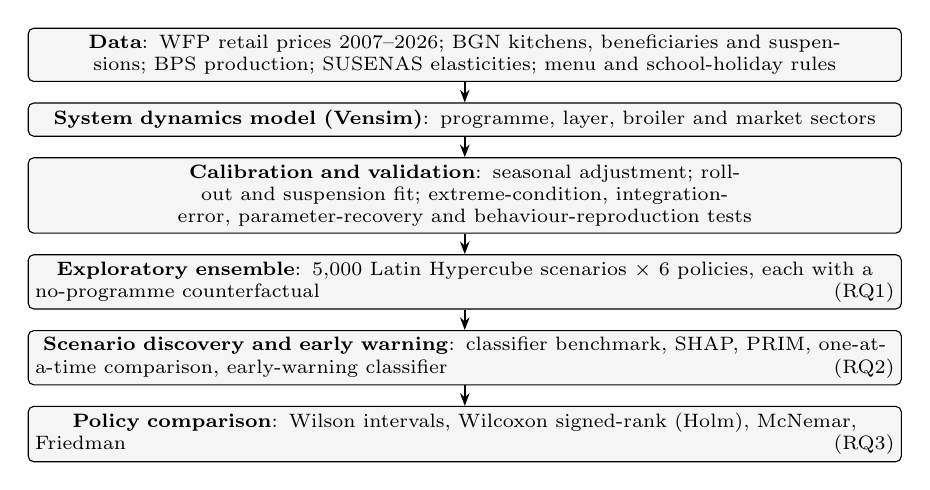
\begin{tikzpicture}[node distance=2.6mm, box/.style={draw, rounded corners=2pt, align=center, font=\scriptsize,
  text width=0.9\linewidth, inner sep=2.5pt, fill=gray!8}, arr/.style={-{Stealth[length=1.6mm]}, semithick}]
\node[box] (d) {\textbf{Data}: WFP retail prices 2007--2026; BGN kitchens, beneficiaries and suspensions;
 BPS production; SUSENAS elasticities; menu and school-holiday rules};
\node[box, below=of d] (m) {\textbf{System dynamics model (Vensim)}: programme, layer, broiler and market sectors};
\node[box, below=of m] (c) {\textbf{Calibration and validation}: seasonal adjustment; roll-out and suspension fit;
 extreme-condition, integration-error, parameter-recovery and behaviour-reproduction tests};
\node[box, below=of c] (e) {\textbf{Exploratory ensemble}: 5,000 Latin Hypercube scenarios
 $\times$ 6 policies, each with a no-programme counterfactual \hfill (RQ1)};
\node[box, below=of e] (s) {\textbf{Scenario discovery and early warning}: classifier benchmark, SHAP, PRIM,
 one-at-a-time comparison, early-warning classifier \hfill (RQ2)};
\node[box, below=of s] (p) {\textbf{Policy comparison}: Wilson intervals, Wilcoxon signed-rank (Holm), McNemar,
 Friedman \hfill (RQ3)};
\foreach \a/\b in {d/m, m/c, c/e, e/s, s/p} \draw[arr] (\a) -- (\b);
\end{tikzpicture}
\end{adjustbox}
\caption{Research framework}\label{fig:framework}
\end{figure}

\subsection{Model Structure}

The model has four interacting sectors simulated weekly from January 2024 to December 2029 (312 weeks, Euler integration with a time step of 0.03125 week). The step is one-sixteenth of the shortest time constant, the half-week minimum delivery time that limits sales when demand jumps as schools reopen, and school-holiday dates are rounded to the nearest 1/16 week so that both time steps in the integration tests switch meals on and off at the same moments. Figure \ref{fig:cld} shows the main feedback loops, Figure \ref{fig:sfd} the stock-and-flow structure, and Appendix \ref{app:eq} lists all equations.


\noindent\textbf{Programme sector.} Planned kitchens (SPPG) follow a logistic roll-out whose final size, midpoint and steepness were fitted to BGN's reported counts of operational kitchens. Kitchens open after an opening delay and can be suspended; the weekly suspension fraction rises when the opening rate exceeds a sustainable opening capacity, representing strain on supervision, staff and suppliers during rapid scaling, and suspended kitchens reopen after a reinstatement time. Beneficiaries served equal operational kitchens times beneficiaries per kitchen, which follows the reported ratio up to September 2026 and then moves to an uncertain future level. Programme demand equals beneficiaries served times the menu quantity per beneficiary times a school-calendar factor: meals pause during school holidays, except for pregnant and breastfeeding mothers and young children until BGN stopped holiday distribution to all groups in June 2026 ~\cite{holiday2026}. Egg demand per beneficiary is the serving size times the number of egg servings per week, which rises from two to at least three on 8 June 2026 ~\cite{egg3x2026}.


\noindent\textbf{Egg (layer) sector.} Pullets are placed and mature into laying hens through a third-order rearing delay. Hens leave the flock through culling and disease outbreaks. Farmers place pullets to replace expected losses and to close the gap between desired and actual flock size, with a partial correction for pullets already in rearing (the supply-line weight ~\cite{sterman2000}). Desired flock size responds to the expected margin, formed by smoothing the market price over an expectation delay (balancing loop B1). Placements are limited by hatchery capacity.


\noindent\textbf{Broiler sector.} Day-old chicks are placed and harvested after grow-out. Placements follow smoothed demand, an inventory correction and the expected margin, limited by day-old-chick supply.


\noindent\textbf{Market and price formation.} For each commodity, market inventory accumulates production and is depleted by sales and spoilage; programme kitchens are served before households when stock is short. Household demand responds to price through a constant own-price elasticity (balancing loop B2). Price adjusts toward an indicated price that rises when inventory coverage is below normal and is pulled toward unit cost plus a normal margin, bounded by a maximum relative price that represents imports, substitutes and market operations. Unit cost depends on the feed price, which rises with the total flock (balancing loop B3) and with exogenous feed-price shocks. Under menu flexibility (policy P4), kitchens substitute other proteins when prices are high, closing a further balancing loop (B4).


\begin{figure*}[!t]
\centering
\begin{adjustbox}{max width=\textwidth}

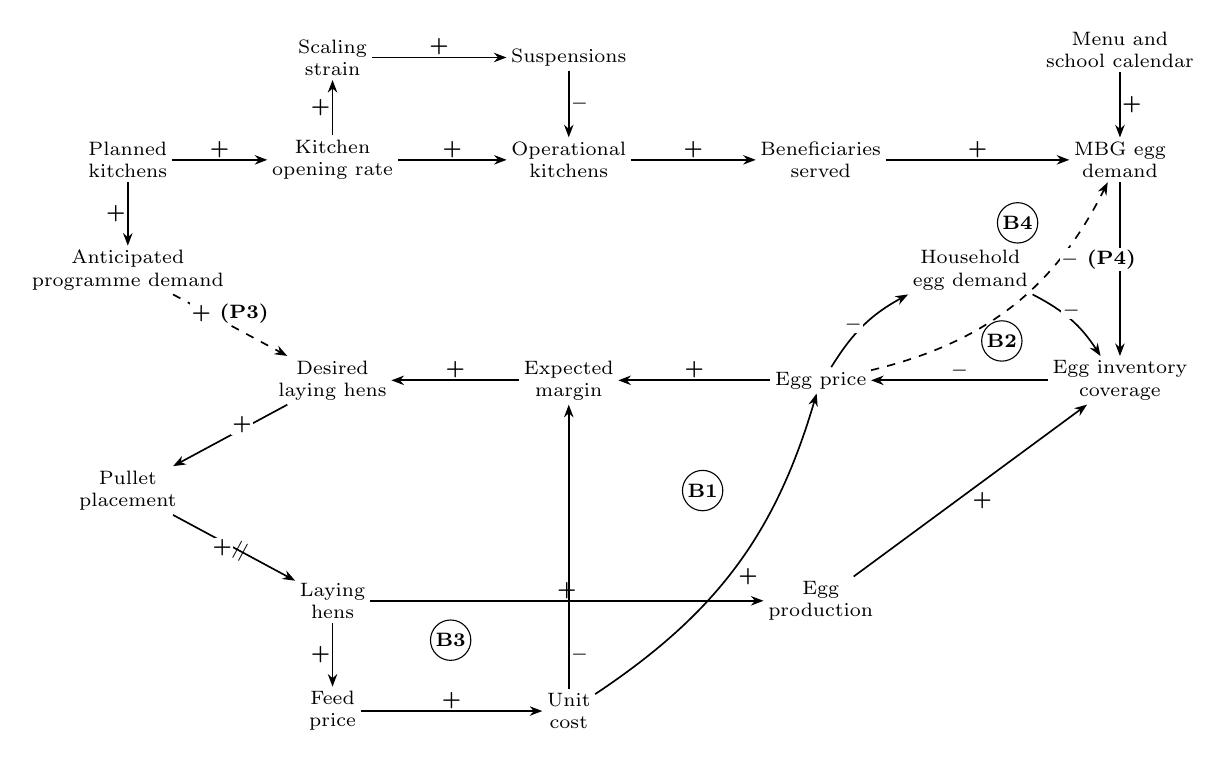
\begin{tikzpicture}[font=\scriptsize, v/.style={align=center, inner sep=1.5pt},
  a/.style={-{Stealth[length=1.6mm]}, semithick}, lab/.style={font=\scriptsize\bfseries, fill=white, inner sep=0.5pt},
  loop/.style={font=\scriptsize\bfseries, circle, draw, inner sep=1pt}]
\node[v] (plan) at (0,3.2) {Planned\\kitchens};
\node[v] (open) at (2.6,3.2) {Kitchen\\opening rate};
\node[v] (oper) at (5.6,3.2) {Operational\\kitchens};
\node[v] (strain) at (2.6,4.5) {Scaling\\strain};
\node[v] (susp) at (5.6,4.5) {Suspensions};
\node[v] (ben) at (8.8,3.2) {Beneficiaries\\served};
\node[v] (mbg) at (12.6,3.2) {MBG egg\\demand};
\node[v] (cal) at (12.6,4.6) {Menu and\\school calendar};
\node[v] (cov) at (12.6,0.4) {Egg inventory\\coverage};
\node[v] (price) at (8.8,0.4) {Egg price};
\node[v] (hh) at (10.7,1.8) {Household\\egg demand};
\node[v] (marg) at (5.6,0.4) {Expected\\margin};
\node[v] (des) at (2.6,0.4) {Desired\\laying hens};
\node[v] (place) at (0,-1.0) {Pullet\\placement};
\node[v] (hens) at (2.6,-2.4) {Laying\\hens};
\node[v] (prod) at (8.8,-2.4) {Egg\\production};
\node[v] (feed) at (2.6,-3.8) {Feed\\price};
\node[v] (cost) at (5.6,-3.8) {Unit\\cost};
\node[v] (ant) at (0,1.8) {Anticipated\\programme demand};
\draw[a] (plan) -- node[lab, above]{+} (open);
\draw[a] (open) -- node[lab, above]{+} (oper);
\draw[a] (open) -- node[lab, left]{+} (strain);
\draw[a] (strain) -- node[lab, above]{+} (susp);
\draw[a] (susp) -- node[lab, right]{$-$} (oper);
\draw[a] (oper) -- node[lab, above]{+} (ben);
\draw[a] (ben) -- node[lab, above]{+} (mbg);
\draw[a] (cal) -- node[lab, right]{+} (mbg);
\draw[a] (mbg) -- node[lab, right]{$-$} (cov);
\draw[a] (cov) -- node[lab, above]{$-$} (price);
\draw[a] (price) to[bend left=15] node[lab, left]{$-$} (hh);
\draw[a] (hh) to[bend left=15] node[lab, above]{$-$} (cov);
\draw[a] (price) -- node[lab, above]{+} (marg);
\draw[a] (marg) -- node[lab, above]{+} (des);
\draw[a] (des) -- node[lab, above right]{+} (place);
\draw[a] (place) -- node[lab, left]{+} node[pos=0.55, sloped]{$||$} (hens);
\draw[a] (hens) -- node[lab, above]{+} (prod);
\draw[a] (prod) -- node[lab, below right]{+} (cov);
\draw[a] (hens) -- node[lab, left]{+} (feed);
\draw[a] (feed) -- node[lab, above]{+} (cost);
\draw[a] (cost) -- node[lab, right, pos=0.12]{$-$} (marg);
\draw[a] (cost) to[bend right=20] node[lab, below right]{+} (price);
\draw[a] (plan) -- node[lab, left]{+} (ant);
\draw[a, dashed] (ant) -- node[lab, above]{+ (P3)} (des);
\draw[a, dashed] (price) to[bend right=25] node[lab, right, pos=0.72]{$-$ (P4)} (mbg);
\node[loop] at (7.3,-1.0) {B1};
\node[loop] at (11.1,0.9) {B2};
\node[loop] at (4.1,-2.9) {B3};
\node[loop] at (11.3,2.4) {B4};
\end{tikzpicture}
\end{adjustbox}
\caption{Causal loop diagram of the egg chain (the broiler chain is analogous). Dashed links act only under policies P3 (forward contracts) and P4 (menu flexibility); $||$ marks the rearing delay}\label{fig:cld}
\end{figure*}

\begin{figure*}[!t]
\centering
\begin{adjustbox}{max width=\textwidth}

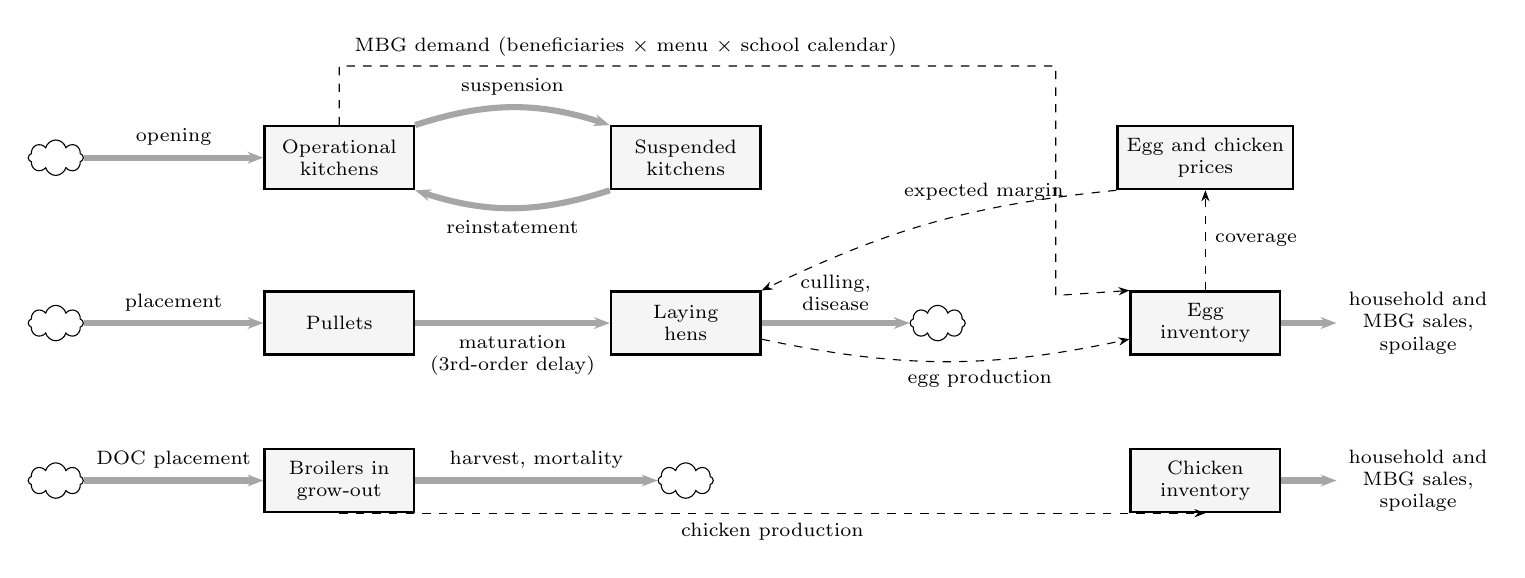
\begin{tikzpicture}[font=\scriptsize, st/.style={draw, thick, minimum width=1.9cm, minimum height=0.8cm, align=center,
  fill=gray!8}, cl/.style={cloud, draw, cloud puffs=8, minimum width=0.7cm, minimum height=0.45cm, inner sep=0pt},
  fl/.style={-{Stealth[length=2mm]}, line width=2.2pt, draw=gray!70}, fll/.style={font=\scriptsize, align=center},
  inf/.style={-{Stealth[length=1.4mm]}, thin, dashed}]
% programme
\node[cl] (c0) at (0,3) {};
\node[st] (op) at (3.6,3) {Operational\\kitchens};
\node[st] (su) at (8.0,3) {Suspended\\kitchens};
\draw[fl] (c0) -- node[fll, above]{opening} (op);
\draw[fl] (op.north east) to[bend left=18] node[fll, above]{suspension} (su.north west);
\draw[fl] (su.south west) to[bend left=18] node[fll, below]{reinstatement} (op.south east);
% layers
\node[cl] (c1) at (0,0.9) {};
\node[st] (pu) at (3.6,0.9) {Pullets};
\node[st] (lh) at (8.0,0.9) {Laying\\hens};
\node[cl] (c2) at (11.2,0.9) {};
\draw[fl] (c1) -- node[fll, above]{placement} (pu);
\draw[fl] (pu) -- node[fll, below]{maturation\\(3rd-order delay)} (lh);
\draw[fl] (lh) -- node[fll, above]{culling,\\disease} (c2);
% broilers
\node[cl] (c3) at (0,-1.1) {};
\node[st] (br) at (3.6,-1.1) {Broilers in\\grow-out};
\node[cl] (c4) at (8.0,-1.1) {};
\draw[fl] (c3) -- node[fll, above]{DOC placement} (br);
\draw[fl] (br) -- node[fll, above]{harvest, mortality} (c4);
% markets

\node[st] (ei) at (14.6,0.9) {Egg\\inventory};
\node[st] (ci) at (14.6,-1.1) {Chicken\\inventory};
\node[st] (ep) at (14.6,3) {Egg and chicken\\prices};

\draw[inf] (lh) to[bend right=12] node[fll, below, pos=0.6]{egg production} (ei);
\draw[inf] (br.south) |- node[fll, below, pos=0.75]{chicken production} (ci.south);
\draw[fl] (ei.east) -- ++(0.7,0) node[right, fll]{household and\\MBG sales,\\spoilage};
\draw[fl] (ci.east) -- ++(0.7,0) node[right, fll]{household and\\MBG sales,\\spoilage};
\draw[inf] (ei.north) -- node[fll, right]{coverage} (ep.south);
\draw[inf] (op.north) -- ++(0,0.75) -| node[fll, pos=0.2, above]{MBG demand (beneficiaries $\times$ menu $\times$ school calendar)} (12.7,1.25) -- (ei.north west);
\draw[inf] (ep.south west) to[bend right=10] node[fll, above, pos=0.35]{expected margin} (lh.north east);
\end{tikzpicture}
\end{adjustbox}
\caption{Simplified stock-and-flow structure (stocks as boxes, flows as thick arrows, information links and production rates computed from stocks dashed). Expected prices and the feed price are omitted for clarity}\label{fig:sfd}
\end{figure*}

\subsection{Policies}

\begin{table}[!htb]
\centering
\footnotesize
\caption{Policy levers}\label{tab:policies}
\begin{tabularx}{\linewidth}{l>{\raggedright\arraybackslash}p{1.9cm}>{\raggedright\arraybackslash}X}
\toprule
\textbf{} & \textbf{Policy} & \textbf{Implementation in the model} \\
\midrule
P0 & Baseline & Current roll-out; cooperative sourcing share 0.1; no forward contracts; fixed menu \\
P1 & Phased roll-out & Roll-out steepness multiplied by 1.75 (a slower S-curve) \\
P2 & Cooperative sourcing & Direct purchase share from farmer groups 0.6 (lower intermediary mark-up) \\
P3 & Forward contracts & 80\% of future programme demand contracted 20 weeks ahead, so farmers can expand flocks before the demand arrives \\
P4 & Menu flexibility & Up to 50\% substitution of other proteins when the relative price exceeds 1.15 \\
P5 & Combined & P2 + P3 + P4 \\
\bottomrule
\end{tabularx}
\end{table}

P1 slows the roll-out so that 10--90\% of kitchens open over about 13 months instead of about 7. P2 reflects the finding that MBG procurement runs largely through intermediaries ~\cite{ipb2026,ambarwati2025}. P4 formalises the reactive menu changes of November 2025 ~\cite{prabowo2025} as a rule.


\subsection{Validation}

Following Barlas ~\cite{barlas1996} and Sterman ~\cite{sterman2000}, the model was subjected to dimensional consistency checks; six extreme-condition tests (no programme, ten-fold programme demand, loss of all laying hens, no hatchery expansion, doubled feed price and near-instant roll-out); an integration-error test comparing the baseline run at two time steps; an ensemble robustness test repeating all ensemble scenarios for four policies at both time steps; a parameter-recovery test applying the calibration procedure to synthetic data with known parameters; and behaviour reproduction against historical prices, assessed with MAPE, $R^2$ and Theil inequality statistics ~\cite{sterman1984}.


\subsection{Exploratory Ensemble and Outcome Indicators}

5,000 scenarios were drawn by Latin Hypercube sampling ~\cite{mckay1979} over 23 uncertain parameters (Table \ref{tab:unc}). Each policy was run on the same scenarios (common random numbers), giving a paired design, and each scenario was also run without the programme. To make the ensemble feasible at the small time step, blocks of scenarios were integrated together as arrays with the same Euler update as PySD; before use, these runs were checked against ordinary PySD runs (21 runs, maximum relative difference 8e-15). Price effects were measured as the difference between the two runs, so that movements caused by exogenous shocks are not attributed to the programme. Outcome indicators were the peak programme-attributable egg and chicken price rise, weeks above the threshold, mean household consumption loss, farmers' margin volatility, protein cost per portion and programme coverage in the final year. A run was labelled a spike if the programme-attributable price rise in either commodity exceeded 10 percentage points of the baseline price. The threshold is well above the largest seasonal premium in the pre-programme data (chicken prices 5.8\% above trend before Idul Fitri; Section \ref{sec:seas}), so a spike is a rise beyond normal seasonal variation; for eggs it corresponds to about Rp 2,814 per kilogram.


\begin{table}[!htb]
\centering
\scriptsize
\caption{Uncertain parameters and ranges}\label{tab:unc}
\begin{tabularx}{\linewidth}{>{\raggedright\arraybackslash}p{2.6cm}rr>{\raggedright\arraybackslash}X}
\toprule
\textbf{Parameter} & \textbf{Low} & \textbf{High} & \textbf{Basis} \\
\midrule
Rollout midpoint & 86 & 100 & Fitted value \$\textbackslash{}pm\$ about 7 weeks \\
Rollout steepness & 5 & 12 & Fitted value \$\textbackslash{}pm\$ about 50\% \\
Target kitchens & 2.4e+04 & 3.2e+04 & Fitted 29,000; BGN targets up to 32,000 \\
Future beneficiaries per kitchen & 1,900 & 2,900 & Sep. 2026 ratio to earlier ratio; cap 2,500--3,000 ~\cite{cap2025} \\
Egg serving size & 0.05 & 0.065 & One egg, 50--65 g \\
Egg servings after menu change & 2 & 4 & Two to four per week ~\cite{egg3x2026} \\
Chicken per beneficiary & 0.08 & 0.26 & Conflicting official estimates ~\cite{gopan2025} \\
Price expectation delay & 4 & 16 & Not identifiable (Table \ref{tab:ident}) \\
Investment sensitivity & 0.5 & 3 & Around calibrated value \\
Supply line weight & 0.1 & 1 & Full range ~\cite{sterman2000} \\
Hatchery capacity factor & 1.1 & 2 & Spare hatchery capacity \\
DOC capacity factor & 1.05 & 1.4 & Day-old-chick oversupply 1.05--1.4 \\
Household egg elasticity & -1 & -0.5 & QUAIDS estimates ~\cite{khoiriyah2024} \\
Household chicken elasticity & -1.8 & -1.2 & QUAIDS estimates ~\cite{khoiriyah2024} \\
Price sensitivity to coverage & 0.5 & 3 & Not identifiable (Table \ref{tab:ident}) \\
Feed shock magnitude & 0 & 0.5 & Up to +50\% feed price \\
Outbreak loss fraction & 0 & 0.3 & Up to 30\% of hens lost \\
Base suspension fraction & 0.002 & 0.008 & Fitted 0.0042; 0.5--2 times \\
Strain sensitivity & 0 & 5 & No data; wide range \\
Kitchen opening delay & 2 & 8 & No data; 2--8 weeks \\
Sustainable opening capacity & 150 & 700 & No data; wide range \\
Intermediary margin & 0.1 & 0.3 & BPS trade margins for eggs 13--27\% \\
Maximum relative price & 2 & 4 & Imports, substitutes, market operations \\
\bottomrule
\end{tabularx}
\end{table}

\subsection{Scenario Discovery and Early Warning}

Using baseline-policy runs, four classifiers (logistic regression, a depth-3 decision tree, a random forest ~\cite{breiman2001} and gradient boosting) were trained to predict spikes from the uncertain parameters and evaluated by stratified five-fold cross-validation. The decision tree provides readable rules; SHAP values on the random forest quantify each parameter's contribution and direction; PRIM identifies a region of the uncertainty space with a high spike density: the box with the highest coverage whose density is at least halfway between the ensemble spike share and one (a fixed target such as 0.8 would select the whole space when spikes are already that common), reporting dimensions restricted by at least 10\% of their range. The results were compared with a one-at-a-time sensitivity analysis. An early-warning classifier was trained on indicators observable 13 weeks after programme start: relative prices, inventory coverage, growth in pullet placements, the kitchen opening rate, the share of suspended kitchens and the feed price.


\subsection{Policy Comparison}

For each policy, spike probability is reported with Wilson 95\% confidence intervals ~\cite{wilson1927}, together with the median and 90th percentile of each outcome. Each policy is compared with P0 on the same scenarios with the Wilcoxon signed-rank test ~\cite{wilcoxon1945}, Holm-corrected ~\cite{holm1979}, with the matched-pairs rank-biserial correlation as effect size ~\cite{kerby2014}; spike occurrence is compared with an exact McNemar test ~\cite{mcnemar1947}, and all policies jointly with the Friedman test ~\cite{friedman1937}.


\section{Data}\label{sec:data}

Table \ref{tab:data} summarises the data used to build, calibrate and validate the model. Appendix \ref{app:par} lists every parameter with its value and source.


\begin{table}[!htb]
\centering
\scriptsize
\caption{Overview of data sources}\label{tab:data}
\begin{tabularx}{\linewidth}{>{\raggedright\arraybackslash}p{2.2cm}>{\raggedright\arraybackslash}X>{\raggedright\arraybackslash}p{1.9cm}>{\raggedright\arraybackslash}p{1.3cm}}
\toprule
\textbf{Data} & \textbf{Source} & \textbf{Use in the model} & \textbf{Period} \\
\midrule
Retail prices of eggs and chicken & WFP market prices ~\cite{wfp} & Calibration; baseline prices; seasonality & 2007--2026 \\
Operational SPPG & BGN ~\cite{bgn2025,bgnaug2025} and press reports ~\cite{sppgpress} & Roll-out fit & Jan. 2025--Sep. 2026 \\
Beneficiaries & BGN ~\cite{bgn2025,antara2026,bgnaug2025}; Kemenkeu ~\cite{sppgpress} & Beneficiaries per kitchen & Jan. 2025--Sep. 2026 \\
Kitchen suspensions & BGN & Suspension hazard & to May 2026 \\
Egg and chicken production & BPS ~\cite{bpsprod} & Initial production & 2024 \\
Household price elasticities & QUAIDS on SUSENAS ~\cite{khoiriyah2024} & Household demand & 2021 \\
Menu and holiday rules & BGN statements ~\cite{bgnegg2025,egg3x2026,holiday2026} & Programme demand & 2025--2026 \\
Biological and cost parameters & Breed standard ~\cite{lohmann}; Indonesian farm and trade statistics & Production and unit cost & various \\
\bottomrule
\end{tabularx}
\end{table}

\subsection{Prices and Seasonality}\label{sec:seas}

Monthly retail prices of chicken eggs and chicken meat were taken from the World Food Programme's Indonesia food price dataset ~\cite{wfp}, which covers about 200 markets. Because the set of reporting markets varies, each market's price was expressed relative to its own 2024 mean, and the national index for each month is the median of these relatives. Months with fewer than 100 reporting markets, and the incomplete latest month, were excluded, leaving 29 monthly observations from January 2024 to October 2026. Baseline prices were set to the 2024 mean of monthly national medians (Rp 28,140/kg for eggs and Rp 35,704/kg for chicken).


The model contains no seasonal household demand, so seasonality was removed before calibration. Using the WFP national series for 2007--2023 (March 2020 to December 2021 excluded), the log ratio of price to its centred 12-month moving average was regressed on calendar-month dummies and on the shares of the 30 days before and after Idul Fitri falling in each month, with HAC standard errors ~\cite{neweywest1987}. Before Idul Fitri, egg prices are 3.6\% above trend (p = 0.002) and chicken prices 5.8\% above trend (p \textless{} 0.001). The fitted seasonal factors were divided out of the 2024--2026 series.


\subsection{Programme Data}

Operational SPPG counts were compiled for 13 dates from January 2025 to September 2026 from BGN releases and press reports of BGN statements ~\cite{bgn2025,bgnaug2025,sppgpress}. Reported beneficiaries per operational kitchen were about 2,700--3,200 until February 2026 but about 2,000 in September 2026 (53--57 million beneficiaries in 27,485 kitchens) ~\cite{sppgpress}; the model follows the observed ratio and treats the later level as uncertain, bounded by BGN's cap of 2,500 portions per kitchen (3,000 with certified cooks) ~\cite{cap2025}. Suspension parameters were fitted to BGN's report that 8,182 SPPG had been suspended at some point and 2,213 remained inactive at the end of May 2026, giving a weekly suspension hazard of about 0.4\% and a mean reinstatement time of about 15 weeks.


Egg servings follow BGN's planning assumption of two egg dishes a week ~\cite{bgnegg2025} until 8 June 2026 and at least three afterwards ~\cite{egg3x2026}. No menu specification for chicken has been published, and official estimates of programme chicken demand conflict, from about 0.04 to 0.26 kg per beneficiary per week ~\cite{gopan2025}; chicken quantity is therefore treated as a deep uncertainty. Initial production was set from BPS 2024 figures: 6,342,705 t of eggs and 3,835,917 t of broiler meat (preliminary) ~\cite{bpsprod}. Household own-price elasticities were set from QUAIDS estimates on SUSENAS 2021 data ($-0.669$ for eggs and $-1.581$ for poultry) ~\cite{khoiriyah2024}. Layer parameters (point of lay at about 18 weeks, laying period of about 65 weeks, hen-day production of about 84.5\%) follow the breed standard ~\cite{lohmann} and Indonesian farm practice; feed is 60--70\% of production cost and trader mark-ups follow BPS trade and transport margins for eggs (13--27\% in 2017--2021).


\subsection{Calibration}

The investment sensitivities of layer and broiler farmers were estimated jointly on the seasonally adjusted egg and chicken series by minimising the sum of squared errors (Nelder--Mead, four starting points). Two further parameters, the price-expectation delay and the sensitivity of price to inventory coverage, are not identifiable from these data: the fit error changes little across wide ranges of either (Table \ref{tab:ident}). They were fixed at 8 weeks and 1.0, values that do not depend on the data, and explored over wide ranges in the ensemble.


\section{Results}\label{sec:results}

\subsection{Validation and Calibration}\label{sec:val}

All six extreme-condition tests passed (Table \ref{tab:val}). The integration-error test gave a maximum difference of 0.63\% of each variable's range between time steps of 0.03125 and 0.015625 week (within the 1\% criterion), and 99.7\% of ensemble runs received the same spike classification at both time steps. The parameter-recovery test recovered all parameters within 1.7\% of their true values. The calibrated layer investment sensitivity is 2.80; the broiler investment sensitivity is 0.000, at the lower bound of zero.


On the seasonally adjusted series the model reproduces egg prices with a MAPE of 3.1\% and an $R^2$ of 0.45, and chicken prices with a MAPE of 4.1\% and an $R^2$ of 0.57 (Table \ref{tab:beh}, Figure \ref{fig:beh}). The bias proportion of the error ($U_M$) is 0.026 for eggs and 0.000 for chicken, and most of the error is unsystematic ($U_C$ = 0.67 and 0.61).


\begin{table*}[!t]
\centering
\scriptsize
\caption{Validation tests}\label{tab:val}
\begin{tabularx}{\linewidth}{>{\raggedright\arraybackslash}X>{\raggedright\arraybackslash}X>{\raggedright\arraybackslash}p{3.2cm}l}
\toprule
\textbf{Test} & \textbf{Pass criterion} & \textbf{Observed} & \textbf{Result} \\
\midrule
A1 No programme -\textgreater{} system stays in equilibrium & max |relative egg price - 1| \textless{} 1e-6 & 0.00e+00 & Pass \\
A2 10x programme demand -\textgreater{} price up, household consumption down & peak price \textgreater{} 1.2 and household ratio \textless{} 0.9; finite, no negative stocks & peak=2.68, hh\_min=0.52 & Pass \\
A3 Outbreak kills 100\% of hens -\textgreater{} production collapses, price spikes, no negatives & min hens \textless{} 10\% of initial; 1.5 \textless{} peak price \textless{}= ceiling; no negative stocks & min hens=3,358,814, peak=3.00 & Pass \\
A4 No hatchery expansion possible -\textgreater{} higher prices than baseline & mean price (weeks 100-312) above baseline run & 1.118 vs 1.015 & Pass \\
A5 Feed price doubles -\textgreater{} egg price rises during shock & price at week 140 above baseline run & 1.090 vs 1.007 & Pass \\
A6 Near-instant roll-out (steepness 0.5 wk) -\textgreater{} more suspensions than baseline (scaling strain) & peak suspended kitchens above baseline run & 5,410 vs 3,177 & Pass \\
B1 Integration error: TIME STEP 0.03125 vs 0.015625 & max |difference| \textless{} 1\% of each variable's range & 0.6328\% & Pass \\
B2 Ensemble robustness: TIME STEP 0.03125 vs 0.015625 (5000 scenarios x 4 policies) & same spike classification in \textgreater{}= 98\% of runs & 99.7\% agree; median |peak diff| 0.0003 & Pass \\
\bottomrule
\end{tabularx}
\end{table*}

\begin{table}[!htb]
\centering
\scriptsize
\caption{Identifiability profile: fit error when one fixed parameter is varied}\label{tab:ident}
\begin{tabularx}{\linewidth}{>{\raggedright\arraybackslash}Xrr}
\toprule
\textbf{Fixed parameter} & \textbf{Value} & \textbf{SSE} \\
\midrule
Price sensitivity to coverage & 0.5 & 0.00460 \\
Price sensitivity to coverage & 1.0 & 0.00402 \\
Price sensitivity to coverage & 2.0 & 0.00391 \\
Price sensitivity to coverage & 3.0 & 0.00394 \\
Price sensitivity to coverage & 5.0 & 0.00393 \\
Price sensitivity to coverage & 10.0 & 0.00396 \\
Price expectation delay & 2.0 & 0.00424 \\
Price expectation delay & 4.0 & 0.00412 \\
Price expectation delay & 8.0 & 0.00402 \\
Price expectation delay & 16.0 & 0.00408 \\
Price expectation delay & 30.0 & 0.00448 \\
\bottomrule
\end{tabularx}
\end{table}

\begin{table}[!htb]
\centering
\scriptsize
\caption{Behaviour reproduction against historical prices}\label{tab:beh}
\begin{tabularx}{\linewidth}{>{\raggedright\arraybackslash}Xrrrrr}
\toprule
\textbf{Series} & \textbf{MAPE} & \textbf{$R^2$} & \textbf{$U_M$} & \textbf{$U_S$} & \textbf{$U_C$} \\
\midrule
egg (seasonally adjusted) & 0.031 & 0.446 & 0.026 & 0.300 & 0.674 \\
chicken (seasonally adjusted) & 0.041 & 0.573 & 0.000 & 0.386 & 0.614 \\
egg (raw, sim x seasonal factor) & 0.031 & 0.261 & 0.022 & 0.044 & 0.934 \\
chicken (raw, sim x seasonal factor) & 0.041 & 0.441 & 0.000 & 0.234 & 0.766 \\
\bottomrule
\end{tabularx}
\end{table}

\begin{figure*}[!t]
\centering
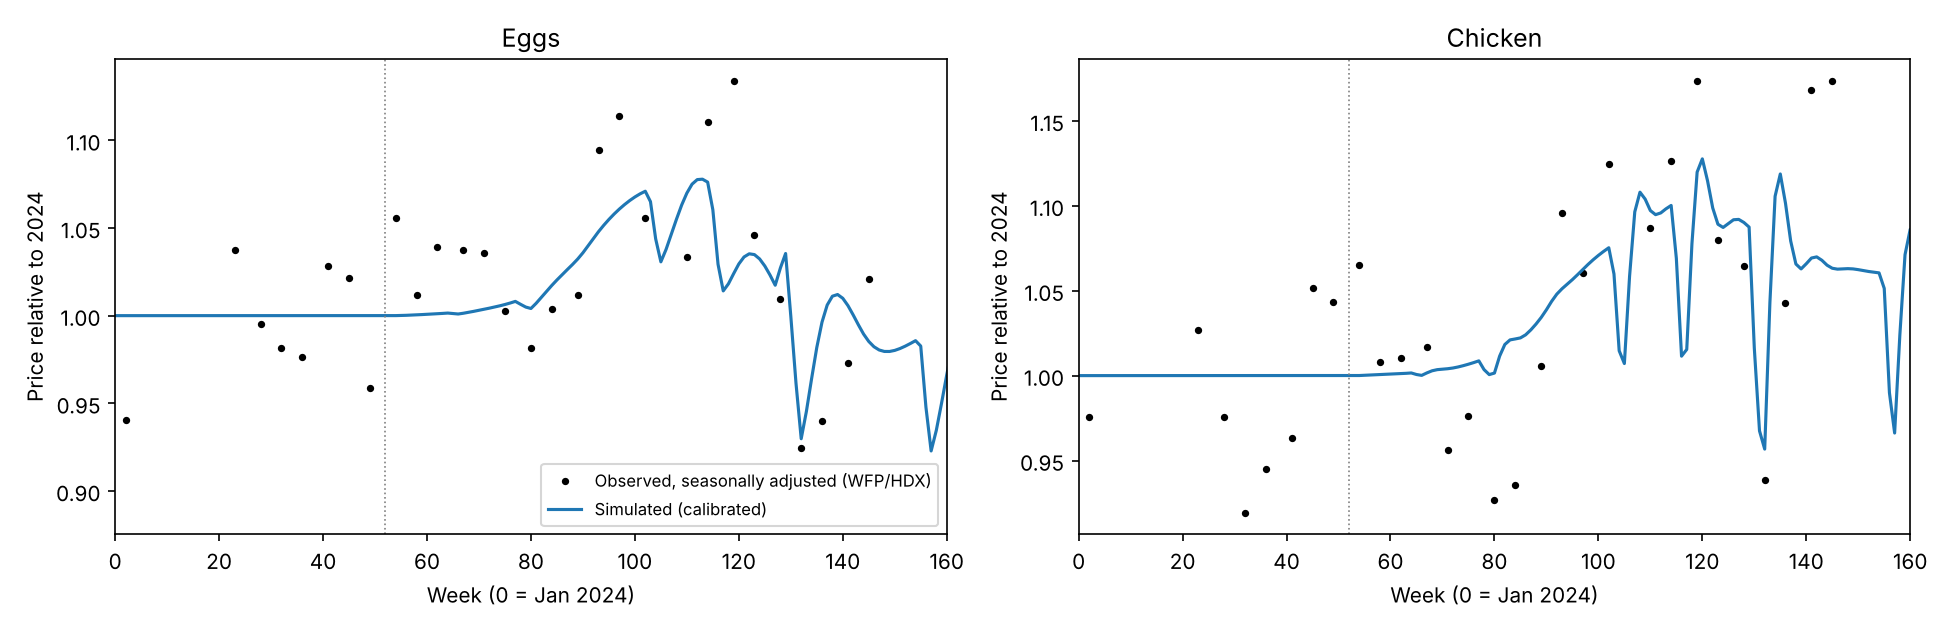
\includegraphics[width=\textwidth]{figures/fig_behaviour_reproduction.png}
\caption{Simulated and observed (seasonally adjusted) relative prices}\label{fig:beh}
\end{figure*}

\subsection{Baseline Dynamics}

Figure \ref{fig:base} compares the calibrated baseline with the same run without the programme. The programme-attributable egg price rise peaks at 11.2 percentage points in April 2029 and the chicken price rise at 12.8 percentage points in April 2026. The egg price exceeds the counterfactual by more than 10 points for 6 weeks and the chicken price for 9 weeks. Average household consumption over the programme period is 1.0\% lower for eggs and 5.8\% lower for chicken than without the programme. School holidays produce short, sharp drops in programme demand that are visible in the price paths.


\begin{figure*}[!t]
\centering
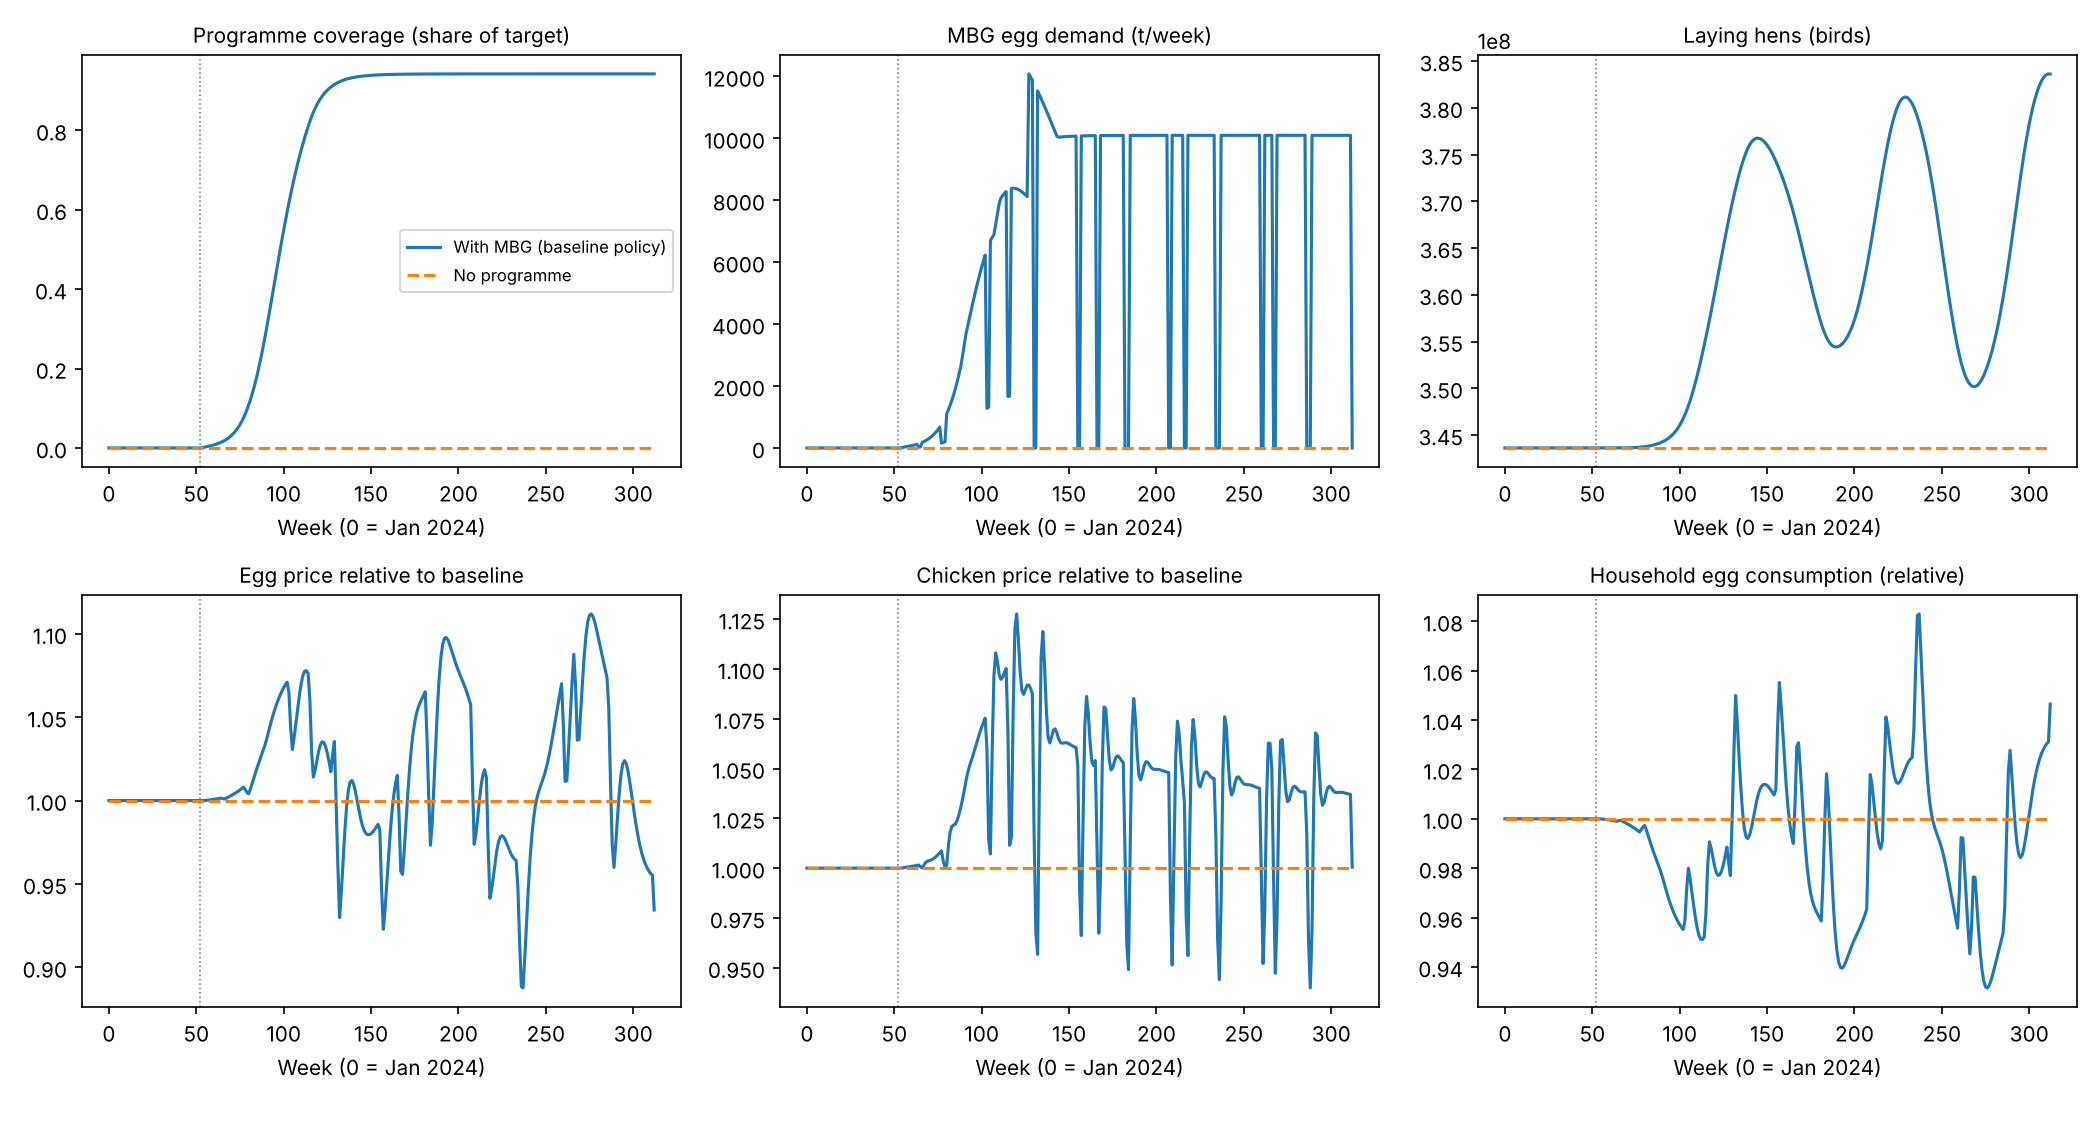
\includegraphics[width=\textwidth]{figures/fig_baseline_dynamics.png}
\caption{Baseline dynamics with and without the programme}\label{fig:base}
\end{figure*}

\subsection{Conditions Leading to Programme-Attributable Spikes}\label{sec:spikes}

Under the baseline policy, 86.0\% of scenarios produce a spike (95\% CI 85.0\%--86.9\%). The spike outcome is predictable from the uncertain inputs: gradient boosting reaches a cross-validated ROC AUC of 0.967, against 0.959 for logistic regression and 0.870 for a depth-3 tree (Table \ref{tab:clf}). The small gap between logistic regression and the tree ensembles shows that interactions between inputs add little: spike risk is largely additive in the uncertain parameters.


SHAP values (Figure \ref{fig:shap}) rank chicken quantity per beneficiary, egg servings per week after June 2026 and size of a disease outbreak as the main drivers. The PRIM box (Table \ref{tab:prim}) covers 80\% of all spikes with a spike density of 94\% (target 93\%), against 86\% in the whole ensemble, and restricts chicken quantity per beneficiary (to 0.128--0.26). The one-at-a-time analysis (Figure \ref{fig:oat}) ranks chicken quantity per beneficiary, size of a disease outbreak, household chicken price elasticity highest; its ranking correlates moderately with the SHAP ranking (Spearman $\rho$ = 0.66). Both identify chicken quantity per beneficiary as the main driver. The rankings differ for second-tier drivers: egg servings per week after June 2026 ranks second by SHAP but sixth one at a time, because one-at-a-time variation measures each effect only with the other inputs at their mid-points, whereas SHAP averages over the whole ensemble.


\begin{table}[!htb]
\centering
\scriptsize
\caption{Spike classifiers (five-fold cross-validation, mean $\pm$ SD)}\label{tab:clf}
\begin{tabularx}{\linewidth}{>{\raggedright\arraybackslash}Xccc}
\toprule
\textbf{Classifier} & \textbf{Accuracy} & \textbf{F1} & \textbf{ROC AUC} \\
\midrule
Logistic regression & 0.921 $\pm$ 0.009 & 0.955 $\pm$ 0.005 & 0.959 $\pm$ 0.008 \\
CART (depth 3) & 0.877 $\pm$ 0.004 & 0.930 $\pm$ 0.003 & 0.870 $\pm$ 0.010 \\
Random forest & 0.903 $\pm$ 0.009 & 0.946 $\pm$ 0.005 & 0.959 $\pm$ 0.005 \\
Gradient boosting & 0.929 $\pm$ 0.010 & 0.960 $\pm$ 0.005 & 0.967 $\pm$ 0.007 \\
\bottomrule
\end{tabularx}
\end{table}

\begin{figure}[!htb]
\centering
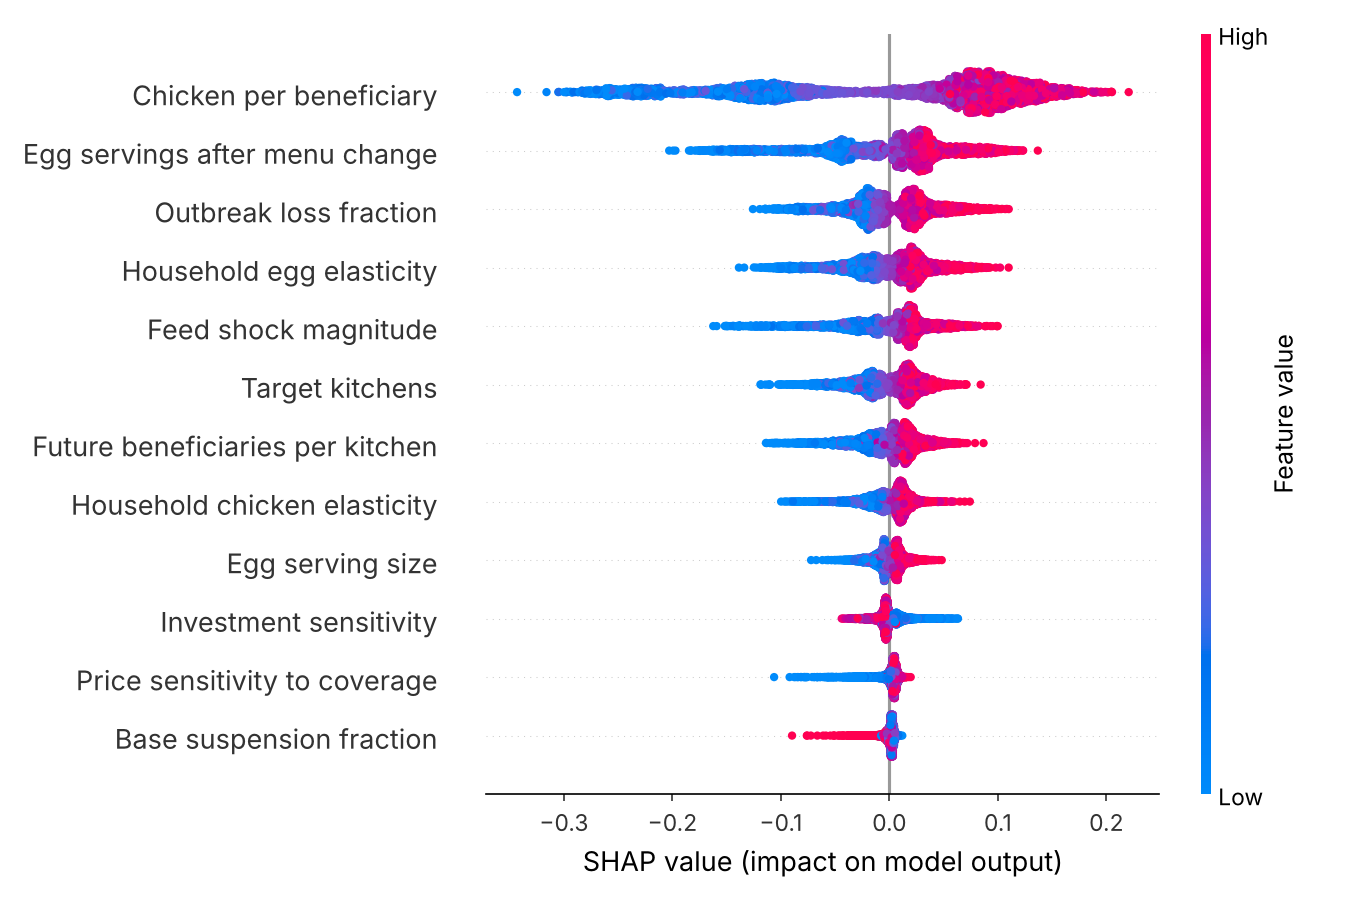
\includegraphics[width=\linewidth]{figures/fig_shap_summary.png}
\caption{SHAP summary for the random-forest spike classifier}\label{fig:shap}
\end{figure}

\begin{table}[!htb]
\centering
\scriptsize
\caption{PRIM box (coverage 0.80, density 0.94, mass 0.73; density target 0.93)}\label{tab:prim}
\begin{tabularx}{\linewidth}{>{\raggedright\arraybackslash}Xrrrr}
\toprule
\textbf{Parameter} & \textbf{Box low} & \textbf{Box high} & \textbf{Full range} & \textbf{Removed} \\
\midrule
Chicken quantity per beneficiary & 0.128 & 0.26 & 0.08--0.26 & 27\% \\
\bottomrule
\end{tabularx}
\end{table}

\begin{figure}[!htb]
\centering
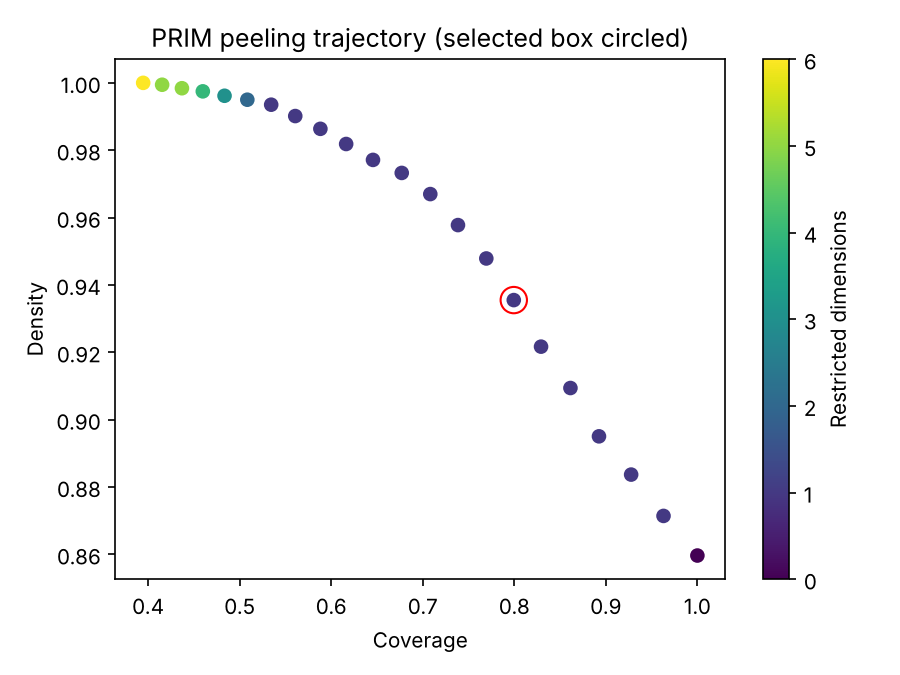
\includegraphics[width=\linewidth]{figures/fig_prim_tradeoff.png}
\caption{PRIM peeling trajectory (coverage versus density)}\label{fig:prim}
\end{figure}

\begin{figure*}[!t]
\centering
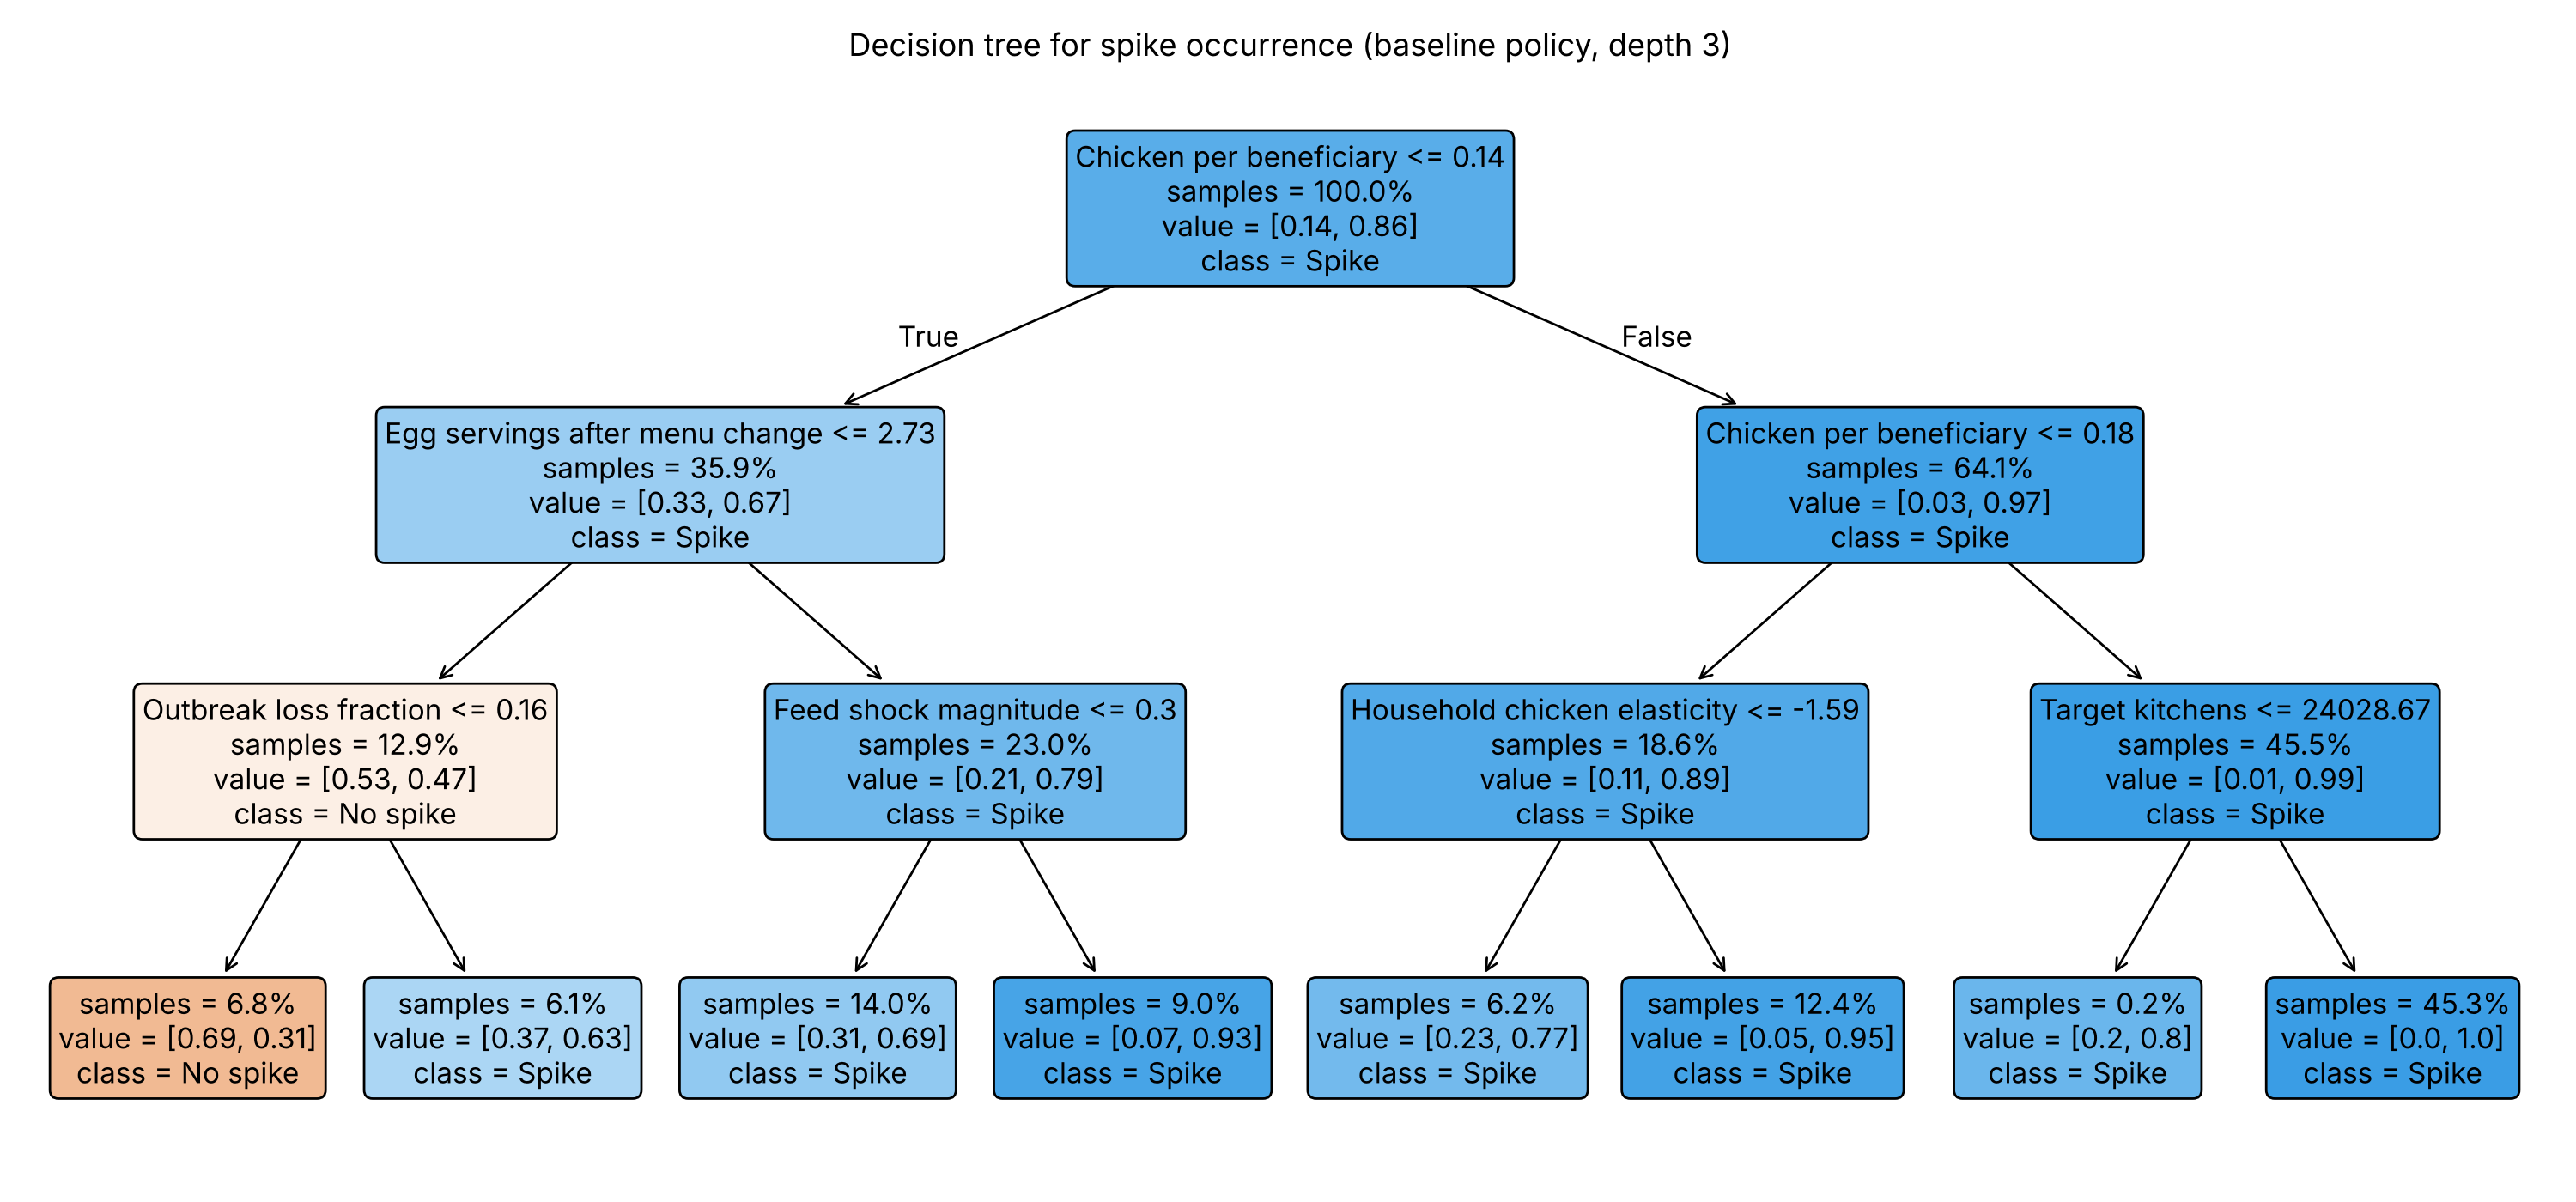
\includegraphics[width=\textwidth]{figures/fig_sd_tree.png}
\caption{Decision tree (depth 3) for spike occurrence under the baseline policy. Each node gives its split, the share of scenarios it contains and the shares without and with a spike [no spike, spike]; left branches satisfy the condition}\label{fig:cart}
\end{figure*}

\begin{figure}[!htb]
\centering
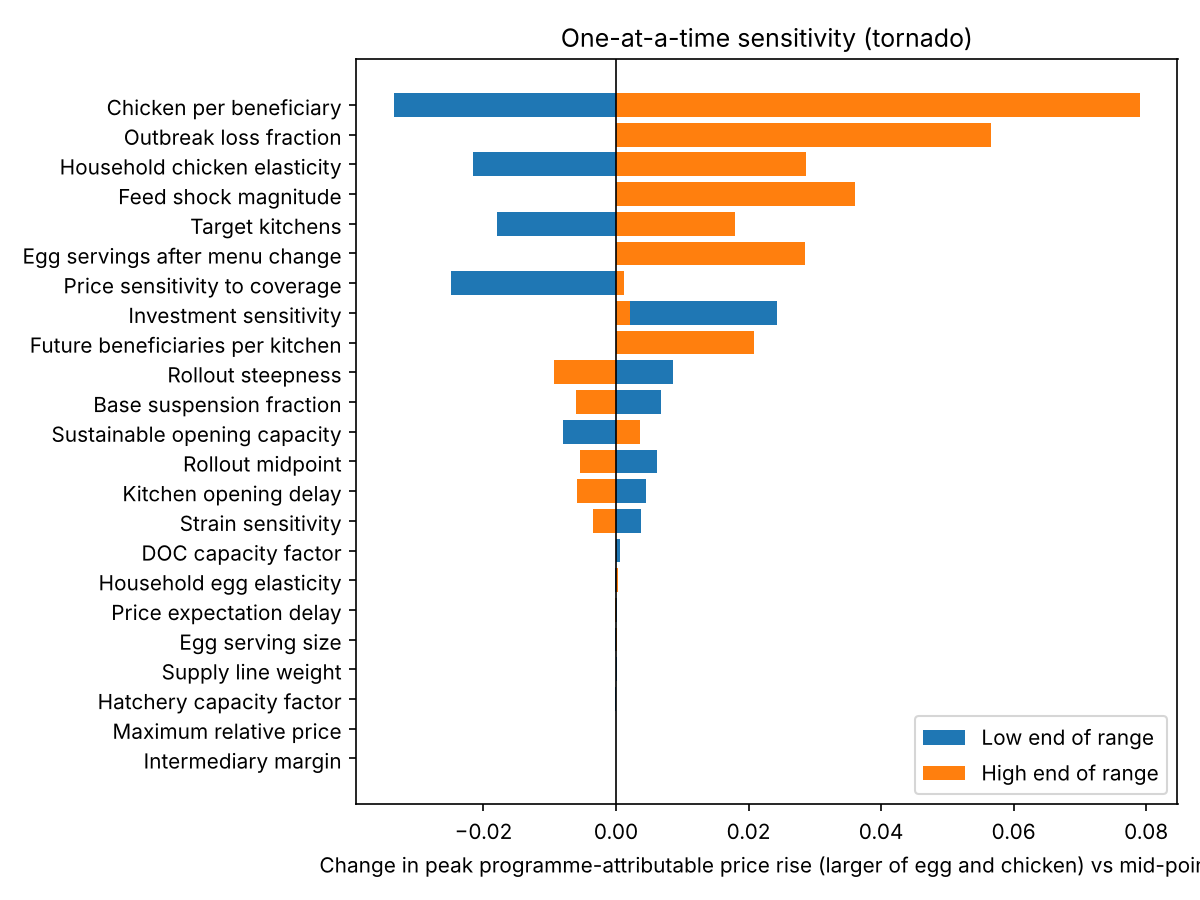
\includegraphics[width=\linewidth]{figures/fig_oat_tornado.png}
\caption{One-at-a-time sensitivity of peak programme-attributable price rise}\label{fig:oat}
\end{figure}

\subsection{Early-Warning Indicators}\label{sec:ew}

Indicators observed 13 weeks after programme start predict later spikes only moderately (Table \ref{tab:ew}): the random forest reaches a ROC AUC of 0.796 and a depth-2 tree 0.613. The first split of the tree uses the chicken coverage (Figure \ref{fig:ewrules}). At that point programme demand is still small relative to supply, so the market signals that would warn of a later spike have not yet formed. Because spikes occur in 86\% of scenarios, accuracy (86\% at best) is no better than always predicting a spike, and every leaf of the depth-2 tree predicts a spike; only the ranking of scenarios by risk, measured by the ROC AUC, carries information.


\begin{table}[!htb]
\centering
\scriptsize
\caption{Early-warning classifiers using indicators observed 13 weeks after programme start}\label{tab:ew}
\begin{tabularx}{\linewidth}{>{\raggedright\arraybackslash}Xccc}
\toprule
\textbf{Classifier} & \textbf{Accuracy} & \textbf{F1} & \textbf{ROC AUC} \\
\midrule
CART (depth 2) & 0.860 & 0.924 & 0.613 \\
Random forest & 0.861 & 0.924 & 0.796 \\
\bottomrule
\end{tabularx}
\end{table}

\begin{figure*}[!t]
\centering
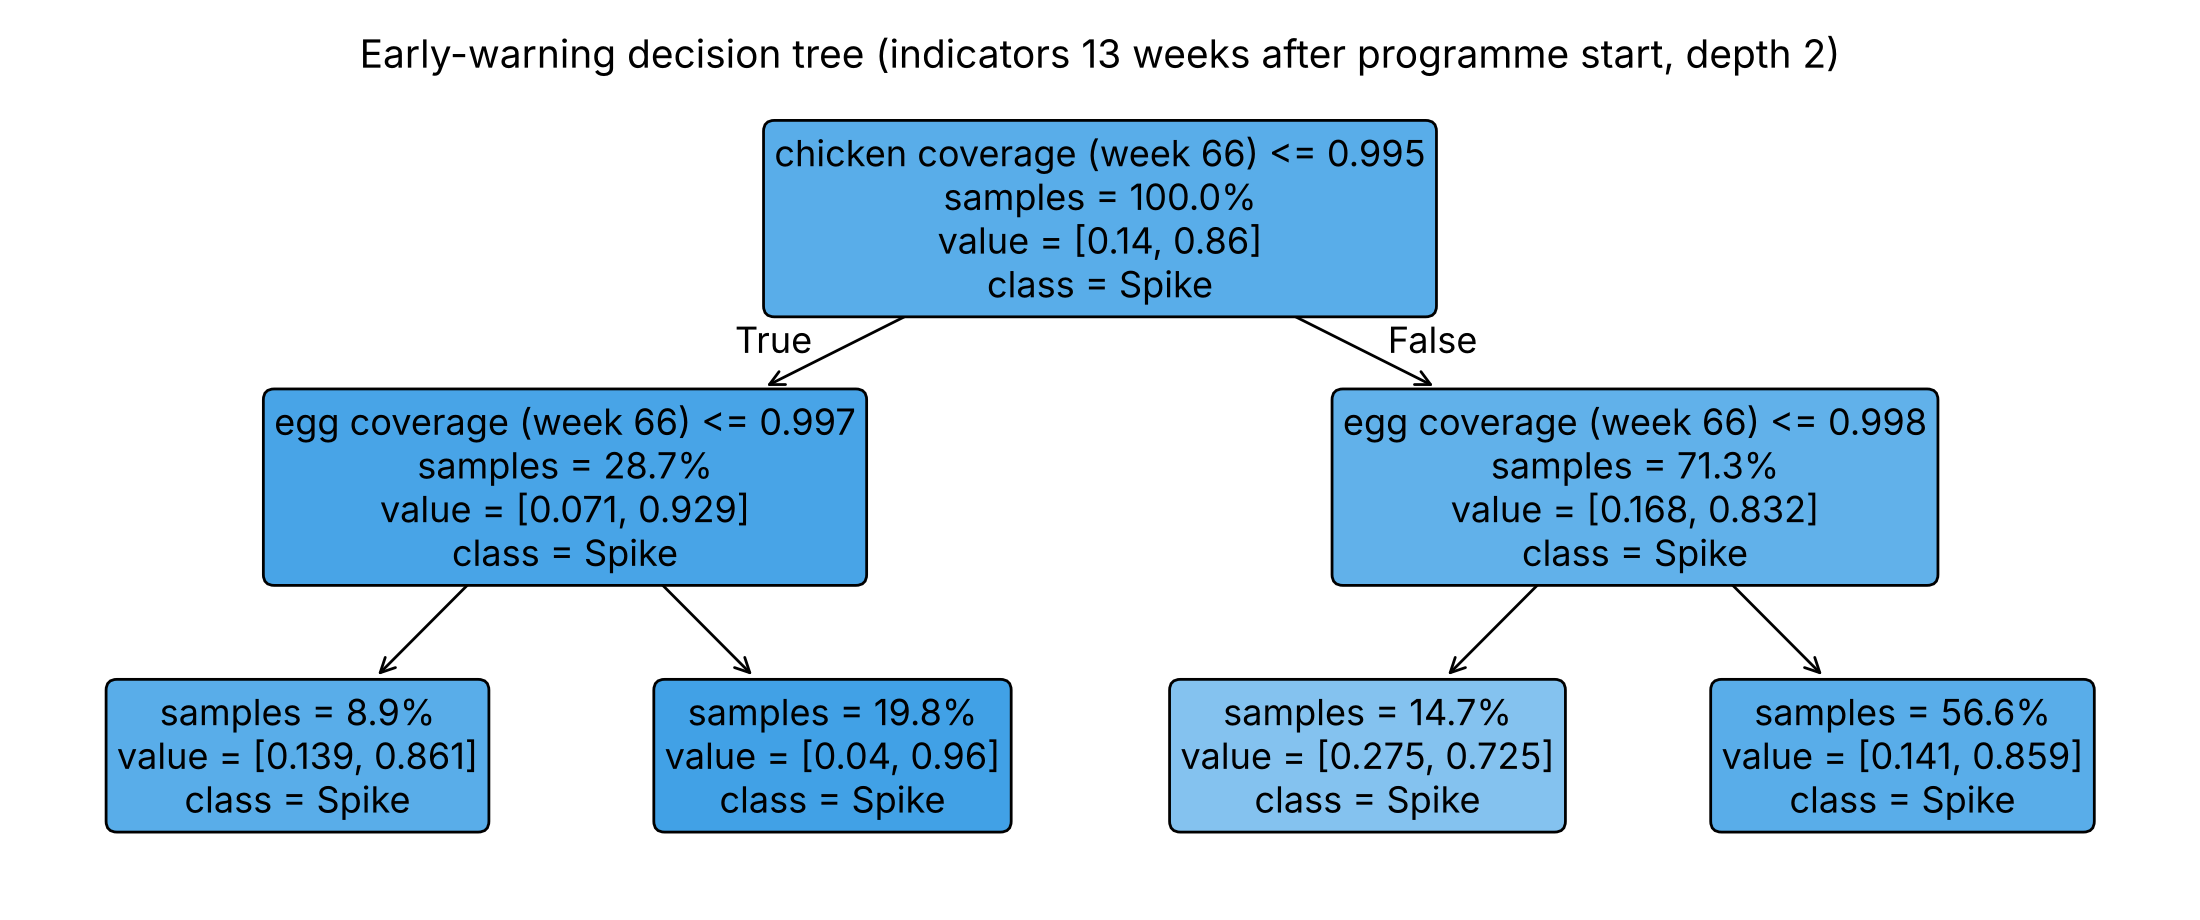
\includegraphics[width=\textwidth]{figures/fig_ew_tree.png}
\caption{Early-warning decision tree (depth 2) using indicators observed 13 weeks after programme start; node contents as in Figure \ref{fig:cart}}\label{fig:ewrules}
\end{figure*}

\subsection{Policy Comparison}\label{sec:policy}

Table \ref{tab:pol} and Figure \ref{fig:pol} compare the policies. Against 86.0\% under P0, the spike probability is P1 (phasing the roll-out) 85.1\%, removing 161 spikes and adding 120; P2 (cooperative sourcing) 86.0\%, removing 0 spikes and adding 0; P3 (forward contracting) 65.7\%, removing 1,137 spikes and adding 122; P4 (menu flexibility) 78.3\%, removing 383 spikes and adding 0; P5 (the combined policy) 38.5\%, removing 2,381 spikes and adding 9 (Table \ref{tab:mcn}). Median protein cost per portion is Rp 2,404 under P0, Rp 2,202 under P2 and Rp 1,973 under P5. Programme coverage in the final year is the same under all policies. After Holm correction, P2 does not differ significantly from P0 on peak egg price, peak chicken price or household egg loss. The Friedman test rejects equal outcomes across policies for every indicator tested (p \textless{} 0.001).


\begin{table*}[!t]
\centering
\scriptsize
\caption{Policy outcomes across scenarios (price effects are programme-attributable relative rises)}\label{tab:pol}
\begin{tabularx}{\linewidth}{l>{\centering\arraybackslash}X>{\centering\arraybackslash}X>{\centering\arraybackslash}X>{\centering\arraybackslash}X>{\centering\arraybackslash}X>{\centering\arraybackslash}X>{\centering\arraybackslash}X>{\centering\arraybackslash}X}
\toprule
\textbf{Policy} & \textbf{Spike prob.} & \textbf{95\% CI} & \textbf{Peak egg (median)} & \textbf{Peak egg (P90)} & \textbf{Peak chicken (median)} & \textbf{Household egg loss} & \textbf{Cost per portion (Rp)} & \textbf{Coverage, final year} \\
\midrule
P0 & 0.860 & 0.850--0.869 & 0.118 & 0.246 & 0.119 & 0.0174 & 2,404 & 0.93 \\
P1 & 0.851 & 0.841--0.861 & 0.128 & 0.277 & 0.111 & 0.0179 & 2,405 & 0.93 \\
P2 & 0.860 & 0.850--0.869 & 0.118 & 0.246 & 0.119 & 0.0174 & 2,202 & 0.93 \\
P3 & 0.657 & 0.643--0.670 & 0.121 & 0.263 & -0.002 & 0.0156 & 2,255 & 0.93 \\
P4 & 0.783 & 0.771--0.794 & 0.094 & 0.141 & 0.119 & 0.0151 & 2,309 & 0.93 \\
P5 & 0.385 & 0.372--0.399 & 0.086 & 0.136 & -0.002 & 0.0130 & 1,973 & 0.93 \\
\bottomrule
\end{tabularx}
\end{table*}

\begin{table}[!htb]
\centering
\scriptsize
\caption{Paired comparison with P0 (Wilcoxon signed-rank)}\label{tab:wil}
\begin{tabularx}{\linewidth}{>{\raggedright\arraybackslash}Xcrrr}
\toprule
\textbf{Outcome} & \textbf{Policy} & \textbf{Median diff.} & \textbf{Rank-biserial r} & \textbf{Holm p} \\
\midrule
Peak egg price & P1 & 0.0073 & 0.508 & $<$0.001 \\
Peak egg price & P2 & 0.0000 & 0.000 & 1.000 \\
Peak egg price & P3 & 0.0044 & 0.160 & $<$0.001 \\
Peak egg price & P4 & -0.0196 & -0.989 & $<$0.001 \\
Peak egg price & P5 & -0.0297 & -0.957 & $<$0.001 \\
Peak chicken price & P1 & -0.0052 & -0.998 & $<$0.001 \\
Peak chicken price & P2 & 0.0000 & 0.000 & 1.000 \\
Peak chicken price & P3 & -0.0992 & -1.000 & $<$0.001 \\
Peak chicken price & P4 & 0.0000 & -0.998 & $<$0.001 \\
Peak chicken price & P5 & -0.0994 & -1.000 & $<$0.001 \\
Household egg loss & P1 & 0.0002 & 0.592 & $<$0.001 \\
Household egg loss & P2 & 0.0000 & 0.000 & 1.000 \\
Household egg loss & P3 & -0.0011 & -0.413 & $<$0.001 \\
Household egg loss & P4 & -0.0020 & -0.768 & $<$0.001 \\
Household egg loss & P5 & -0.0045 & -0.909 & $<$0.001 \\
Cost per portion & P1 & -1.6 & -0.316 & $<$0.001 \\
Cost per portion & P2 & -195.7 & -1.000 & $<$0.001 \\
Cost per portion & P3 & -120.6 & -1.000 & $<$0.001 \\
Cost per portion & P4 & -83.2 & -1.000 & $<$0.001 \\
Cost per portion & P5 & -408.9 & -1.000 & $<$0.001 \\
\bottomrule
\end{tabularx}
\end{table}

\begin{table}[!htb]
\centering
\scriptsize
\caption{Change in spike occurrence relative to P0 (McNemar)}\label{tab:mcn}
\begin{tabular}{lrrr}
\toprule
\textbf{Policy} & \textbf{Spikes removed} & \textbf{Spikes added} & \textbf{$p$ (exact)} \\
\midrule
P1 & 161 & 120 & 0.017 \\
P2 & 0 & 0 & 1.000 \\
P3 & 1,137 & 122 & $<$0.001 \\
P4 & 383 & 0 & $<$0.001 \\
P5 & 2,381 & 9 & $<$0.001 \\
\bottomrule
\end{tabular}
\end{table}

Table \ref{tab:sdef} repeats the comparison under other spike definitions: lower and higher thresholds, and a sustained definition requiring the rise to stay above 10 points for several weeks. P5 and P3 are the two best policies under 4 of the 6 definitions, and most baseline spikes are sustained: 80.5\% of scenarios stay above 10 points for at least four weeks. For severe spikes (above 20 points) the ranking of single policies changes: menu flexibility lowers the probability to 3.8\%, against 19.6\% for forward contracting, because substitution caps how far kitchens keep buying when prices are high.


\begin{table}[!htb]
\centering
\scriptsize
\caption{Spike probability under alternative spike definitions (peak programme-attributable rise above a threshold, or above 10 points for at least 4 or 13 weeks)}\label{tab:sdef}
\begin{tabularx}{\linewidth}{l>{\centering\arraybackslash}X>{\centering\arraybackslash}X>{\centering\arraybackslash}X>{\centering\arraybackslash}X>{\centering\arraybackslash}X>{\centering\arraybackslash}X}
\toprule
\textbf{Policy} & \textbf{Peak \textgreater{}5\%} & \textbf{Peak \textgreater{}10\%} & \textbf{Peak \textgreater{}15\%} & \textbf{Peak \textgreater{}20\%} & \textbf{$\geq$4 wk} & \textbf{$\geq$13 wk} \\
\midrule
P0 & 0.999 & 0.860 & 0.518 & 0.232 & 0.805 & 0.687 \\
P1 & 0.997 & 0.851 & 0.513 & 0.255 & 0.799 & 0.674 \\
P2 & 0.999 & 0.860 & 0.518 & 0.232 & 0.805 & 0.687 \\
P3 & 0.967 & 0.657 & 0.364 & 0.196 & 0.605 & 0.469 \\
P4 & 0.998 & 0.783 & 0.333 & 0.038 & 0.711 & 0.575 \\
P5 & 0.945 & 0.385 & 0.078 & 0.009 & 0.334 & 0.232 \\
\bottomrule
\end{tabularx}
\end{table}

\begin{figure*}[!t]
\centering
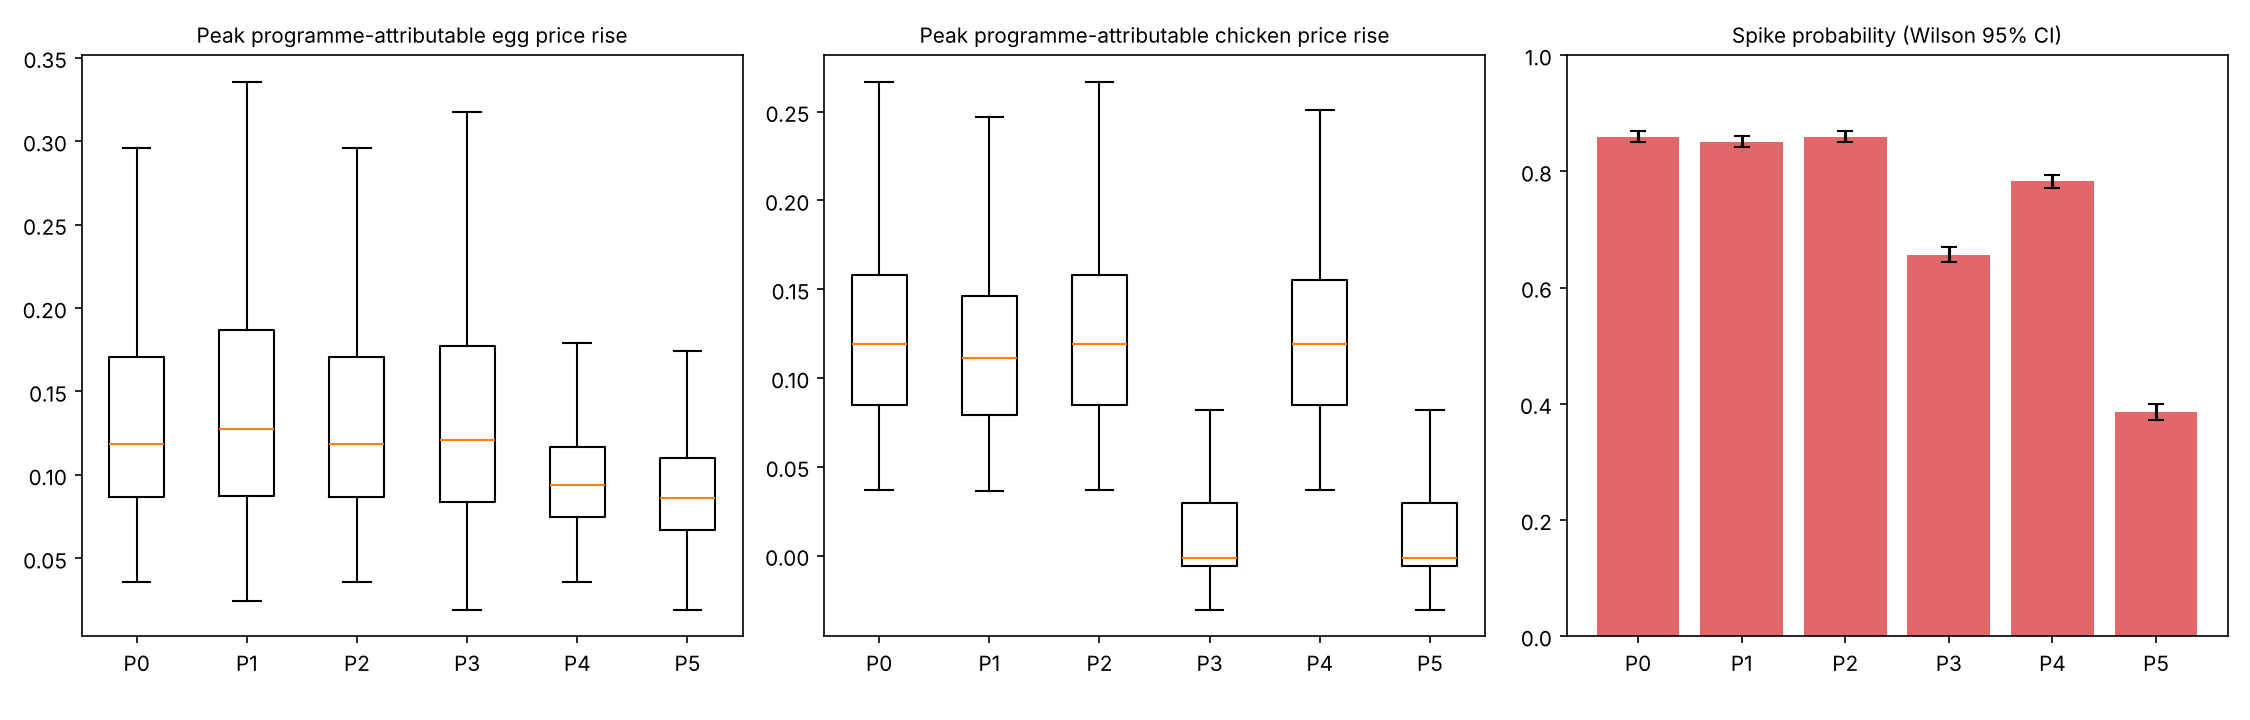
\includegraphics[width=\textwidth]{figures/fig_policy_comparison.png}
\caption{Policy comparison across scenarios}\label{fig:pol}
\end{figure*}

\begin{figure}[!htb]
\centering
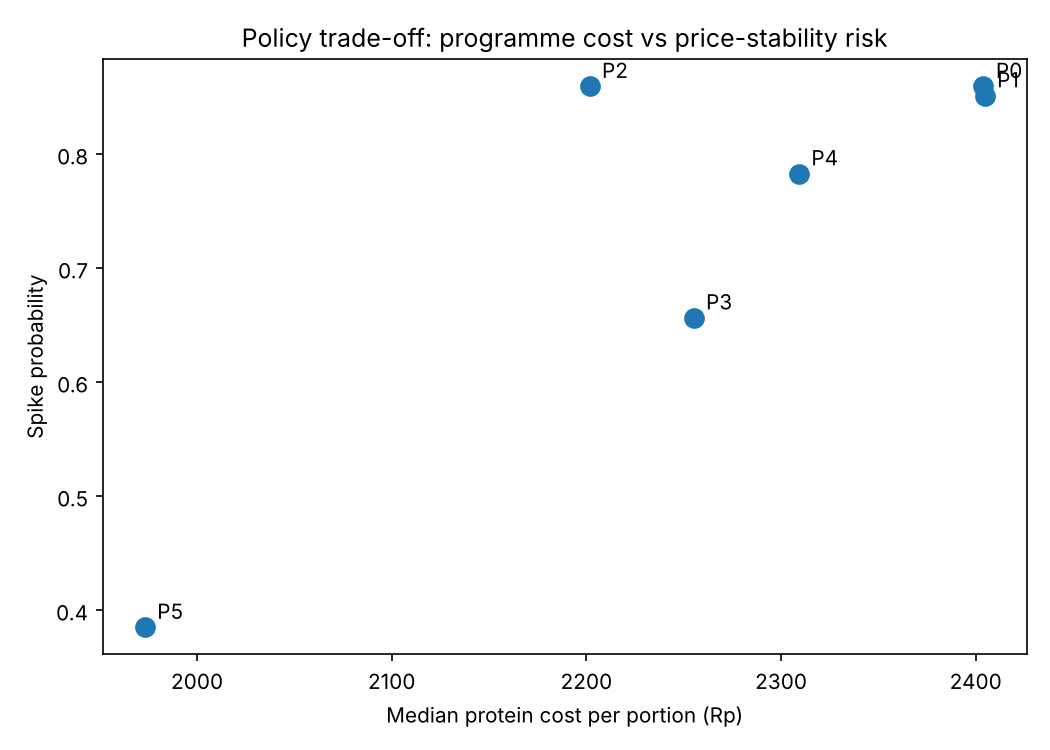
\includegraphics[width=\linewidth]{figures/fig_policy_tradeoff.png}
\caption{Protein cost per portion versus spike probability}\label{fig:trade}
\end{figure}

\section{Discussion}\label{sec:discussion}

\subsection{Why the System Behaves This Way}

Programme demand is set by kitchen numbers, menus and the school calendar, not by price, and it grew from almost nothing to tens of millions of meals within a year. Laying capacity cannot follow at that speed: a pullet placed in response to higher prices starts laying about 18 weeks later, and farmers form price expectations with a delay. In the meantime the market clears through price, and the balancing loop that acts fastest is household demand (B2): households buy fewer eggs and less chicken, which is why the programme-attributable price rise in the baseline coincides with household consumption 1.0\% (eggs) and 5.8\% (chicken) lower than without the programme. The programme's nutritional gain for beneficiaries is therefore partly offset by a loss for non-beneficiary households, a distributional effect that does not appear in programme statistics.


Once new flocks come into lay, the supply loop (B1) overshoots: in the baseline the egg price falls 6.6 percentage points below the counterfactual by December 2029. This is the commodity-cycle mechanism described by Meadows ~\cite{meadows1970} and Sterman ~\cite{sterman2000}, triggered here by a demand shock rather than by a supply shock. It matches the sequence observed in 2026, when farm-gate egg prices fell below the government reference price and BGN raised egg servings to absorb the surplus ~\cite{egg3x2026}.


School holidays act as a second, recurring shock. When meals stop for two to three weeks, programme demand drops at once, but eggs keep coming from flocks sized for term-time demand, so inventories rise and prices fall; when schools reopen, demand returns at full strength. The June 2026 request by the Minister of Agriculture that companies absorb farmers' eggs and chicken during the holiday ~\cite{amran2026} and the price rise he attributed to MBG after schools reopened ~\cite{okezone2026} are both consistent with this mechanism. The June 2026 rule that also stopped holiday meals for mothers and young children ~\cite{holiday2026} deepened these swings.


The broiler chain behaves differently. The calibrated sensitivity of broiler placements to the expected margin is close to zero, meaning that placements follow demand and integrator planning rather than prices. This is consistent with the integrator-dominated structure and quota-based allocation of day-old chicks described by Haryana et al. ~\cite{haryana2026}, and it explains why chicken price risk depends so strongly on how much chicken the programme buys.


\subsection{Comparison with Previous Studies and the Attribution Debate}

The counterfactual design speaks directly to the disagreement between BPS and the Ministry of Agriculture. In October 2025 the seasonally adjusted national egg price was 9.4\% above its 2024 level and the chicken price 9.5\%. In the calibrated baseline, the programme accounts for 5.0 percentage points of the egg price and 5.2 points of the chicken price in that month. The programme therefore explains a substantial part of the October 2025 egg price rise, supporting the BPS interpretation ~\cite{bps2025}, while seasonal factors explain the rest. Neither agency's position can be confirmed from price data alone, because programme demand and seasonal demand rose at the same time; separating them requires a counterfactual.


The results agree with Mitchell, Thompson and Malone ~\cite{mitchell2024} that biological lags determine how far prices move after a shock: in the model the size of the programme-attributable rise depends on how fast demand arrives relative to the rearing delay. They extend Haryana et al. ~\cite{haryana2026}, who show that broiler price instability arises from the structure of supply, by adding a public programme as a new source of demand-side instability. The results are also consistent with the argument of Gelli et al. ~\cite{gelli2021} that the market effects of school meals depend on procurement scale: MBG procurement is large relative to the national egg market, which is why national prices respond. Local effects in less integrated markets may be larger than the national effects estimated here.


\subsection{Practical Implications for Programme Design}\label{sec:implications}

Four implications follow. First, procurement design matters more than roll-out speed. Forward contracts, which let farmers expand flocks before programme demand arrives, reduce spike probability from 86.0\% to 65.7\%, while slowing the roll-out (P1) reduces it only to 85.1\% and creates spikes in 120 scenarios where none occurred before, because a slower roll-out can shift demand into a less favourable phase of the supply cycle. BGN could publish roll-out schedules and menu plans several months ahead and contract a share of eggs and chicken with farmer cooperatives on that basis.


Second, menus should flex by rule rather than by ad hoc decision. Menu flexibility (P4) lowers spike probability to 78.3\% and cuts the 90th percentile of the egg price rise from 24.6 to 14.1 percentage points. The November 2025 and June 2026 menu changes show that BGN already uses menus as a market instrument ~\cite{prabowo2025,egg3x2026}; a published rule linking servings to price thresholds would make the response predictable for farmers.


Third, cooperative sourcing (P2) lowers the protein cost per portion from Rp 2,404 to Rp 2,202 but does not change prices in the model, because it changes who captures the margin, not how much is produced. It is worth pursuing for budget reasons, and its price effect would depend on whether cooperatives also expand supply. Combining the three procurement measures (P5) gives the lowest spike probability (38.5\%) and the lowest cost per portion.


Fourth, the programme should plan for school holidays. Keeping meals for mothers and young children during holidays, aligning holiday periods with government purchasing for food reserves, or shifting part of holiday-period egg supply to processing would reduce the stop-start shock that the June 2026 rules amplified. Because early market indicators predict spikes only moderately, these measures need to be designed in advance rather than triggered by price signals.


\subsection{Methodological Contribution}

The analysis shows what the combination of system dynamics and scenario discovery adds to a single simulation or a one-at-a-time sensitivity analysis. The counterfactual design separates the programme's effect from feed, disease and seasonal shocks that would raise prices anyway, which is the question the agencies disagree on. A one-at-a-time analysis finds the same main driver, but it describes behaviour around a single base case; only the ensemble gives the probability of a spike across the uncertainty space and shows how policies change it. PRIM turns the ensemble into conditions that decision makers can act on, such as the chicken quantity per beneficiary beyond which spikes become likely, and SHAP values show the direction and size of each driver's effect.


\section{Limitations and Future Work}\label{sec:limits}

The study has several limitations. First, the model is national and has no regional detail or trade between regions; local price effects, particularly in eastern Indonesia, may differ from the national effects estimated here. Second, the chicken quantity per beneficiary is not published and official estimates conflict, so it is treated as a wide uncertainty; because it is a leading driver of spikes, publication of menu specifications by BGN would sharpen the results. Third, the temporary substitution of eggs requested in November 2025 is not modelled, because its size and duration were not reported, and the school-holiday calendar is a national approximation. Fourth, cooperative sourcing affects only procurement cost in the model. Fifth, household price elasticities come from a provincial study and are applied nationally, and the kitchen suspension hazard is constant although suspensions occurred in enforcement waves.


Sixth, the model reproduces the main movements of seasonally adjusted prices with moderate accuracy ($R^2$ of 0.45 for eggs and 0.57 for chicken); short-term fluctuations driven by events outside the model, such as weather, disease outbreaks and government market operations, are not reproduced. Two parameters, the price-expectation delay and the price response to inventory coverage, are not identifiable from the available data and were explored over wide ranges instead.


Future work could add regional subscripts and inter-island trade, collect procurement data from a sample of SPPG to replace the menu uncertainty with observed quantities, model cooperative sourcing as a channel for supply expansion, apply behaviour-based scenario discovery ~\cite{steinmann2020} to classify the shape of price paths rather than only their peaks, and extend the model to other programme commodities such as milk, rice and vegetables.


\section{Conclusion}\label{sec:conclusion}

This paper developed a system dynamics model of Indonesia's egg and broiler supply chains under the Free Nutritious Meals programme and analysed it with machine-learning scenario discovery over 5,000 scenarios. On RQ1, the programme's price-inelastic demand meets a biologically delayed supply response, so prices rise until households cut consumption and new flocks arrive; in the calibrated baseline the programme-attributable rise peaks at 11.2 percentage points for eggs and 12.8 for chicken, and school holidays add recurring demand swings. On RQ2, a spike of more than 10 points occurs in 86.0\% of scenarios under current policy and depends mainly on chicken quantity per beneficiary, egg servings per week after June 2026 and size of a disease outbreak; spikes occur in 94\% of scenarios with chicken quantity per beneficiary above 0.128 kg per week. On RQ3, forward contracting is the most effective single policy (65.7\%), and combining cooperative sourcing, forward contracts and menu flexibility reduces spike probability to 38.5\% at a lower cost per portion, without reducing programme coverage.


The contributions are a calibrated dynamic model of programme-driven demand shocks, a counterfactual design that separates programme effects from seasonal and external shocks, and an ensemble analysis that turns thousands of simulations into spike probabilities, thresholds and paired policy comparisons that a single run or a one-at-a-time analysis cannot provide. The results suggest that large public food programmes should plan procurement, menus and holiday supply in advance, because by the time price signals appear the supply response is months away. Extending the model to regional markets and other commodities is the natural next step.


\clearpage

\section*{Declarations}

\noindent\textbf{Funding:} This research received no external funding.


\noindent\textbf{Competing interests:} The author declares no competing interests.


\noindent\textbf{Data and code availability:} The Vensim model, the Python analysis code, the price extract and the programme data with their sources are available from the author's repository (github.com/daniel766hi/kaggle-compe, folder paper/).


\noindent\textbf{Use of AI tools:} An AI assistant (Claude, Anthropic) was used to help develop the simulation and analysis code, collect and process public data, and draft and edit the text. The author reviewed, revised and verified all content, including every equation, data source and reference, and takes full responsibility for the work.


\begin{thebibliography}{99}
\small
\bibitem{bgn2025} Badan Gizi Nasional, ``Awal Januari 2026, BGN operasikan 19.188 SPPG,'' press release, Jan. 2026. [Online]. Available: https://www.bgn.go.id/news/siaran-pers/awal-januari-2026-bgn-operasikan-19188-sppg
\bibitem{antara2026} Antara, ``BGN: 21.897 SPPG sudah beroperasi layani 65 juta penerima manfaat MBG,'' 12 Feb. 2026. [Online]. Available: https://www.antaranews.com/berita/5414198
\bibitem{budget} Kontan, ``Prabowo naikkan anggaran MBG 94,76\% di 2026, tembus Rp 335 triliun,'' Aug. 2025. [Online]. Available: https://nasional.kontan.co.id/news/prabowo-naikkan-anggaran-mbg-9476-di-2026-tembus-rp-335-triliun
\bibitem{meadows1970} D. L. Meadows, \textit{Dynamics of Commodity Production Cycles}. Cambridge, MA: Wright-Allen Press, 1970.
\bibitem{sterman2000} J. D. Sterman, \textit{Business Dynamics: Systems Thinking and Modeling for a Complex World}. Boston, MA: Irwin/McGraw-Hill, 2000.
\bibitem{bps2025} Bisnis.com, ``BPS duga program MBG jadi pemicu inflasi telur dan daging ayam,'' 3 Nov. 2025. [Online]. Available: https://ekonomi.bisnis.com/read/20251103/9/1925640
\bibitem{kementan2025} Bisnis.com, ``Kementan pastikan harga telur dan ayam stabil, pasokan untuk program MBG aman,'' 19 Nov. 2025. [Online]. Available: https://ekonomi.bisnis.com/read/20251119/12/1930149
\bibitem{prabowo2025} Republika, ``Prabowo minta sementara telur ayam di menu MBG diganti telur puyuh,'' 21 Nov. 2025. [Online]. Available: https://news.republika.co.id/berita/t61xeu409
\bibitem{egg3x2026} Detik Finance, ``Menu telur program MBG minimal 3 kali seminggu imbas harga anjlok,'' June 2026. [Online]. Available: https://finance.detik.com/berita-ekonomi-bisnis/d-8522633
\bibitem{amran2026} CNN Indonesia, ``MBG libur, Amran minta perusahaan serap telur-daging ayam peternak,'' 17 June 2026. [Online]. Available: https://www.cnnindonesia.com/ekonomi/20260617180357-92-1370127
\bibitem{okezone2026} Okezone, ``Harga ayam dan telur naik, Mentan sebut efek MBG,'' 27 July 2026. [Online]. Available: https://economy.okezone.com/read/2026/07/27/320/3232582
\bibitem{handbury2021} J. Handbury and S. Moshary, ``School food policy affects everyone: Retail responses to the National School Lunch Program,'' NBER Working Paper 29384, 2021. https://doi.org/10.3386/w29384
\bibitem{gelli2021} A. Gelli, E. Masset, \textit{et al.}, ``School meals as a market for smallholder agriculture: Experimental evidence from Ghana,'' IFPRI Discussion Paper 02045, International Food Policy Research Institute, Washington, DC, 2021.
\bibitem{ipb2026} ``Analisis struktur rantai pasok pangan dan keterlibatan UMKM lokal dalam pelaksanaan program Makan Bergizi Gratis (MBG) di Kota Tangerang Selatan,'' \textit{Jurnal Manajemen dan Organisasi}, vol. 17, no. 3, pp. 275--291, 2026. https://doi.org/10.29244/jmo.v17i3.73792
\bibitem{ambarwati2025} O. C. Ambarwati and H. Kurniawati, ``Strategi pemanfaatan potensi pangan lokal untuk mendukung program Makan Bergizi Gratis di Jawa Tengah,'' \textit{Analisis Kebijakan Pembangunan}, vol. 2, no. 1, pp. 47--60, 2025.
\bibitem{mitchell2024} J. L. Mitchell, J. M. Thompson, and T. Malone, ``Biological lags and market dynamics in vertically coordinated food supply chains: HPAI impacts on U.S. egg prices,'' \textit{Food Policy}, vol. 126, 102655, 2024. https://doi.org/10.1016/j.foodpol.2024.102655
\bibitem{haryana2026} A. Haryana, Suprayogi, R. Wangsaputra, and R. Govindaraju, ``Regional food supply system planning: A system dynamics analysis of broiler chicken supply and price stabilization policies in Indonesia,'' \textit{Journal of Regional and City Planning}, vol. 37, no. 1, pp. 52--96, 2026. https://doi.org/10.5614/jpwk.2026.37.1.3
\bibitem{aboah2022} J. Aboah and D. Enahoro, ``A systems thinking approach to understand the drivers of change in backyard poultry farming system,'' \textit{Agricultural Systems}, vol. 202, 103475, 2022. https://doi.org/10.1016/j.agsy.2022.103475
\bibitem{bryant2010} B. P. Bryant and R. J. Lempert, ``Thinking inside the box: A participatory, computer-assisted approach to scenario discovery,'' \textit{Technological Forecasting and Social Change}, vol. 77, no. 1, pp. 34--49, 2010. https://doi.org/10.1016/j.techfore.2009.08.002
\bibitem{friedman1999} J. H. Friedman and N. I. Fisher, ``Bump hunting in high-dimensional data,'' \textit{Statistics and Computing}, vol. 9, no. 2, pp. 123--143, 1999. https://doi.org/10.1023/A:1008894516817
\bibitem{kwakkel2016} J. H. Kwakkel and M. Jaxa-Rozen, ``Improving scenario discovery for handling heterogeneous uncertainties and multinomial classified outcomes,'' \textit{Environmental Modelling \& Software}, vol. 79, pp. 311--321, 2016. https://doi.org/10.1016/j.envsoft.2015.11.020
\bibitem{steinmann2020} P. Steinmann, W. L. Auping, and J. H. Kwakkel, ``Behavior-based scenario discovery using time series clustering,'' \textit{Technological Forecasting and Social Change}, vol. 156, 120052, 2020. https://doi.org/10.1016/j.techfore.2020.120052
\bibitem{kwakkel2017} J. H. Kwakkel, ``The Exploratory Modeling Workbench: An open source toolkit for exploratory modeling, scenario discovery, and (multi-objective) robust decision making,'' \textit{Environmental Modelling \& Software}, vol. 96, pp. 239--250, 2017. https://doi.org/10.1016/j.envsoft.2017.06.054
\bibitem{breiman2001} L. Breiman, ``Random forests,'' \textit{Machine Learning}, vol. 45, no. 1, pp. 5--32, 2001. https://doi.org/10.1023/A:1010933404324
\bibitem{lundberg2017} S. M. Lundberg and S.-I. Lee, ``A unified approach to interpreting model predictions,'' in \textit{Advances in Neural Information Processing Systems}, vol. 30, 2017.
\bibitem{barlas1996} Y. Barlas, ``Formal aspects of model validity and validation in system dynamics,'' \textit{System Dynamics Review}, vol. 12, no. 3, pp. 183--210, 1996.
\bibitem{pysd} J. Houghton and M. Siegel, ``Advanced data analytics for system dynamics models using PySD,'' in \textit{Proc. 33rd Int. System Dynamics Conf.}, Cambridge, MA, 2015.
\bibitem{holiday2026} CNN Indonesia, ``MBG bumil, busui dan balita ikut disetop sementara saat libur sekolah,'' 19 June 2026. [Online]. Available: https://www.cnnindonesia.com/ekonomi/20260619124748-92-1370802
\bibitem{sterman1984} J. D. Sterman, ``Appropriate summary statistics for evaluating the historical fit of system dynamics models,'' \textit{Dynamica}, vol. 10, no. 2, pp. 51--66, 1984.
\bibitem{mckay1979} M. D. McKay, R. J. Beckman, and W. J. Conover, ``A comparison of three methods for selecting values of input variables in the analysis of output from a computer code,'' \textit{Technometrics}, vol. 21, no. 2, pp. 239--245, 1979. https://doi.org/10.1080/00401706.1979.10489755
\bibitem{cap2025} Detik Finance, ``BGN batasi dapur MBG maksimal siapkan 3.000 porsi per hari,'' Oct. 2025. [Online]. Available: https://finance.detik.com/berita-ekonomi-bisnis/d-8185320
\bibitem{gopan2025} Kontan, ``Produksi ditambah, GOPAN: pasokan ayam masih lebih untuk program MBG,'' Nov. 2025. [Online]. Available: https://industri.kontan.co.id/news/produksi-ditambah-gopan-pasokan-ayam-masih-lebih-untuk-program-mbg
\bibitem{khoiriyah2024} N. Khoiriyah, D. Forgenie, S. Sookhai, and A. J. Saputro, ``Demand elasticities of animal-sourced food: Empirical study in Yogyakarta, Indonesia,'' \textit{International Journal of Food and Agricultural Economics}, vol. 12, no. 3, pp. 171--188, 2024.
\bibitem{wilson1927} E. B. Wilson, ``Probable inference, the law of succession, and statistical inference,'' \textit{Journal of the American Statistical Association}, vol. 22, no. 158, pp. 209--212, 1927. https://doi.org/10.1080/01621459.1927.10502953
\bibitem{wilcoxon1945} F. Wilcoxon, ``Individual comparisons by ranking methods,'' \textit{Biometrics Bulletin}, vol. 1, no. 6, pp. 80--83, 1945. https://doi.org/10.2307/3001968
\bibitem{holm1979} S. Holm, ``A simple sequentially rejective multiple test procedure,'' \textit{Scandinavian Journal of Statistics}, vol. 6, no. 2, pp. 65--70, 1979.
\bibitem{kerby2014} D. S. Kerby, ``The simple difference formula: An approach to teaching nonparametric correlation,'' \textit{Comprehensive Psychology}, vol. 3, 2014. https://doi.org/10.2466/11.IT.3.1
\bibitem{mcnemar1947} Q. McNemar, ``Note on the sampling error of the difference between correlated proportions or percentages,'' \textit{Psychometrika}, vol. 12, no. 2, pp. 153--157, 1947. https://doi.org/10.1007/BF02295996
\bibitem{friedman1937} M. Friedman, ``The use of ranks to avoid the assumption of normality implicit in the analysis of variance,'' \textit{Journal of the American Statistical Association}, vol. 32, no. 200, pp. 675--701, 1937. https://doi.org/10.1080/01621459.1937.10503522
\bibitem{wfp} World Food Programme, ``Indonesia -- Food Prices,'' Humanitarian Data Exchange, licence CC BY-IGO. [Online]. Available: https://data.humdata.org/dataset/72cc0659-142b-41af-821a-cb981a852617 (accessed 7 Nov. 2026).
\bibitem{bgnaug2025} Badan Gizi Nasional, ``Program MBG sentuh 15 juta penerima manfaat, BGN bidik 82,9 juta pada akhir 2025,'' press release, Aug. 2025. [Online]. Available: https://www.bgn.go.id/news/siaran-pers/program-mbg-sentuh-15-juta-penerima-manfaat-bgn-bidik-829-juta-pada-akhir-2025
\bibitem{sppgpress} Press reports of BGN statements on operational SPPG, 2025--2026: Bisnis.com (24 June and 28 Sep. 2025), Investortrust (8 Sep. 2025), CNN Indonesia (16 Sep. 2025), Kompas TV (18 June 2026) and Kementerian Keuangan via RM.id (Oct. 2026). Full list with URLs in the data repository.
\bibitem{bpsprod} Badan Pusat Statistik, ``Produksi Telur Ayam Petelur menurut Provinsi (Ton), 2024'' and ``Produksi Daging Ayam Ras Pedaging menurut Provinsi (Ton), 2024,'' preliminary figures, Jakarta, 2025.
\bibitem{bgnegg2025} Bisnis.com, ``Kepala BGN wanti-wanti RI bisa krisis telur buat penuhi MBG,'' 8 Apr. 2025. [Online]. Available: https://ekonomi.bisnis.com/read/20250408/12/1867518
\bibitem{lohmann} Lohmann Breeders, \textit{Lohmann Brown-Classic Layers: Management Guide}. Cuxhaven, Germany: Lohmann Breeders GmbH.
\bibitem{neweywest1987} W. K. Newey and K. D. West, ``A simple, positive semi-definite, heteroskedasticity and autocorrelation consistent covariance matrix,'' \textit{Econometrica}, vol. 55, no. 3, pp. 703--708, 1987. https://doi.org/10.2307/1913610
\end{thebibliography}

\onecolumn
\appendix
\section{Model Equations}\label{app:eq}
\scriptsize
\begin{longtable}{>{\raggedright\arraybackslash}p{4.2cm}>{\raggedright\arraybackslash\ttfamily}p{8.9cm}>{\raggedright\arraybackslash}p{2.4cm}}
\toprule \textbf{Variable} & \textbf{Equation} & \textbf{Units} \\ \midrule \endhead
INITIAL TIME & 0 & Week \\
FINAL TIME & 312 & Week \\
TIME STEP & 0.03125 & Week [0,?] \\
SAVEPER & 1 & Week [0,?] \\
Programme start time & 53 & Week \\
Target kitchens & 29767 & kitchen \\
Rollout midpoint & 92.05 & Week \\
Rollout steepness & 7.39 & Week \\
Rollout fraction & IF THEN ELSE(Time \textgreater{}= Programme start time, 1 / (1 + EXP(-(Time - Rollout midpoint) / Rollout steepness)), 0) & Dmnl \\
Planned kitchens & Target kitchens * Rollout fraction & kitchen \\
Operational kitchens & INTEG(Kitchen opening rate + Reinstatement rate - Suspension rate, 0) & kitchen \\
Suspended kitchens & INTEG(Suspension rate - Reinstatement rate, 0) & kitchen \\
Kitchen opening delay & 4 & Week \\
Kitchen opening rate & MAX(0, Planned kitchens - Operational kitchens - Suspended kitchens) / Kitchen opening delay & kitchen/Week \\
Reinstatement time & 14.96 & Week \\
Reinstatement rate & Suspended kitchens / Reinstatement time & kitchen/Week \\
Base suspension fraction & 0.00409 & 1/Week \\
Sustainable opening capacity & 300 & kitchen/Week \\
Scaling strain & Kitchen opening rate / Sustainable opening capacity & Dmnl \\
Strain sensitivity & 2 & Dmnl \\
Effect of scaling strain on suspension & 1 + Strain sensitivity * MAX(0, Scaling strain - 1) & Dmnl \\
Suspension rate & Operational kitchens * Base suspension fraction * Effect of scaling strain on suspension & kitchen/Week \\
Beneficiaries per kitchen & IF THEN ELSE(Time \textless{}= Last observed beneficiary week, Observed beneficiaries per kitchen(Time), Observed beneficiaries per kitchen(Last observed beneficiary week) + (Future beneficiaries per kitchen - Observed beneficiaries per kitchen(Last observed beneficiary week)) * MIN(1, (Time - Last observed beneficiary week) / Beneficiary adjustment time)) & person/kitchen \\
Last observed beneficiary week & 143.29 & Week \\
Future beneficiaries per kitchen & 2000 & person/kitchen \\
Beneficiary adjustment time & 26 & Week \\
Beneficiaries served & Operational kitchens * Beneficiaries per kitchen & person \\
Holiday service share & IF THEN ELSE(Time \textgreater{}= Holiday rule change time, 0, Holiday service share before rule change) & Dmnl \\
Holiday service share before rule change & 0.2 & Dmnl \\
Holiday rule change time & 128.625 & Week \\
Programme in session & 1 - School holiday indicator(Time) * (1 - Holiday service share) & Dmnl \\
Programme coverage & ZIDZ(Beneficiaries served, Target kitchens * Beneficiaries per kitchen) & Dmnl \\
Portions per beneficiary & 5 & portion/(person*Week) \\
Egg per beneficiary & Egg serving size * IF THEN ELSE(Time \textgreater{}= Egg menu change time, Egg servings after menu change, Egg servings before menu change) & kg/(person*Week) \\
Egg serving size & 0.06 & kg/serving \\
Egg servings before menu change & 2 & serving/(person*Week) \\
Egg servings after menu change & 3 & serving/(person*Week) \\
Egg menu change time & 127.0 & Week \\
Chicken per beneficiary & 0.18 & kg/(person*Week) \\
Menu flexibility switch & 0 & Dmnl \\
Max menu substitution & 0.5 & Dmnl \\
Substitution price threshold & 1.15 & Dmnl \\
Egg menu multiplier & 1 - Menu flexibility switch * Max menu substitution * MIN(1, MAX(0, (Relative egg price - Substitution price threshold) / 0.2)) & Dmnl \\
Chicken menu multiplier & 1 - Menu flexibility switch * Max menu substitution * MIN(1, MAX(0, (Relative chicken price - Substitution price threshold) / 0.2)) & Dmnl \\
MBG egg demand & Beneficiaries served * Egg per beneficiary * Egg menu multiplier * Programme in session / 1000 & t/Week \\
MBG chicken demand & Beneficiaries served * Chicken per beneficiary * Chicken menu multiplier * Programme in session / 1000 & t/Week \\
Forward contract share & 0 & Dmnl \\
Contract lead time & 20 & Week \\
Anticipated rollout fraction & IF THEN ELSE(Time + Contract lead time \textgreater{}= Programme start time, 1 / (1 + EXP(-(Time + Contract lead time - Rollout midpoint) / Rollout steepness)), 0) & Dmnl \\
Anticipated MBG egg demand & Target kitchens * Anticipated rollout fraction * Beneficiaries per kitchen * Egg per beneficiary / 1000 & t/Week \\
Anticipated MBG chicken demand & Target kitchens * Anticipated rollout fraction * Beneficiaries per kitchen * Chicken per beneficiary / 1000 & t/Week \\
Cooperative sourcing share & 0.1 & Dmnl \\
Intermediary margin & 0.2 & Dmnl \\
Egg procurement price & Egg price * (1 + Intermediary margin * (1 - Cooperative sourcing share)) & Rp/kg \\
Chicken procurement price & Chicken price * (1 + Intermediary margin * (1 - Cooperative sourcing share)) & Rp/kg \\
Programme protein cost & (MBG egg sales * Egg procurement price + MBG chicken sales * Chicken procurement price) * 1000 & Rp/Week \\
Protein cost per portion & Programme protein cost / MAX(1, Beneficiaries served * Portions per beneficiary) & Rp/portion \\
Feed shock magnitude & 0 & Dmnl \\
Feed shock time & 120 & Week \\
Feed shock duration & 26 & Week \\
Exogenous feed price index & 1 + Feed shock magnitude * PULSE(Feed shock time, Feed shock duration) & Dmnl \\
Broiler feed weight & 0.5 & Dmnl \\
Total birds & Laying hens + Pullets + Broilers in growout * Broiler feed weight & bird \\
Initial total birds & INITIAL(Total birds) & bird \\
Feed price sensitivity to flock & 0.3 & Dmnl \\
Relative feed price & Exogenous feed price index * (Total birds / Initial total birds) \textasciicircum{} Feed price sensitivity to flock & Dmnl \\
Egg mass & 0.06 & kg/egg \\
Lay rate & 5.9 & egg/(bird*Week) \\
Production per hen & Lay rate * Egg mass / 1000 & t/(bird*Week) \\
Initial egg production & 121640 & t/Week \\
Initial laying hens & Initial egg production / Production per hen & bird \\
Productive life & 65 & Week \\
Rearing time & 18 & Week \\
Laying hens & INTEG(Maturation - Culling - Disease loss, Initial laying hens) & bird \\
Pullets & INTEG(Pullet placement - Maturation, Initial laying hens / Productive life * Rearing time) & bird \\
Maturation & DELAY3(Pullet placement, Rearing time) & bird/Week \\
Culling & Laying hens / Productive life & bird/Week \\
Outbreak loss fraction & 0 & Dmnl \\
Outbreak time & 150 & Week \\
Outbreak duration & 4 & Week \\
Disease loss & Laying hens * (-LN(1 - MIN(Outbreak loss fraction, 0.999))) * PULSE(Outbreak time, Outbreak duration) / Outbreak duration & bird/Week \\
Egg production & Laying hens * Production per hen & t/Week \\
Egg spoilage fraction & 0.01 & 1/Week \\
Normal egg coverage & 2 & Week \\
Reference household egg demand & Initial egg production / (1 + Egg spoilage fraction * Normal egg coverage) & t/Week \\
Egg inventory & INTEG(Egg production - Egg sales - Egg spoilage, Reference household egg demand * Normal egg coverage) & t \\
Egg spoilage & Egg inventory * Egg spoilage fraction & t/Week \\
Minimum delivery time & 0.5 & Week \\
Egg available & Egg inventory / Minimum delivery time & t/Week \\
Household egg elasticity & -0.669 & Dmnl \\
Household egg demand & Reference household egg demand * Relative egg price \textasciicircum{} Household egg elasticity & t/Week \\
MBG egg sales & MIN(MBG egg demand, Egg available) & t/Week \\
Household egg sales & MIN(Household egg demand, Egg available - MBG egg sales) & t/Week \\
Egg sales & MBG egg sales + Household egg sales & t/Week \\
Total egg demand & MBG egg demand + Household egg demand & t/Week \\
Relative egg coverage & (Egg inventory / MAX(1, Total egg demand)) / Normal egg coverage & Dmnl \\
Baseline egg price & 28140 & Rp/kg \\
Normal egg margin & 0.1 & Dmnl \\
Egg feed cost share & 0.7 & Dmnl \\
Base egg unit cost & Baseline egg price / (1 + Normal egg margin) & Rp/kg \\
Egg unit cost & Base egg unit cost * (Egg feed cost share * Relative feed price + 1 - Egg feed cost share) & Rp/kg \\
Price sensitivity to coverage & 1 & Dmnl \\
Cost pull weight & 0.3 & Dmnl \\
Maximum relative price & 3 & Dmnl \\
Price adjustment time & 2 & Week \\
Indicated egg price & MIN(Maximum relative price * Baseline egg price, Egg price * Relative egg coverage \textasciicircum{} (-Price sensitivity to coverage) * (Egg unit cost * (1 + Normal egg margin) / Egg price) \textasciicircum{} Cost pull weight) & Rp/kg \\
Change in egg price & (Indicated egg price - Egg price) / Price adjustment time & Rp/(kg*Week) \\
Egg price & INTEG(Change in egg price, Baseline egg price) & Rp/kg \\
Relative egg price & Egg price / Baseline egg price & Dmnl \\
Price expectation delay & 8 & Week \\
Expected egg price & SMOOTH(Egg price, Price expectation delay) & Rp/kg \\
Expected egg margin & (Expected egg price - Egg unit cost) / Egg unit cost & Dmnl \\
Egg farmer margin & (Egg price - Egg unit cost) / Egg unit cost & Dmnl \\
Investment sensitivity & 1.5 & Dmnl \\
Effect of margin on desired hens & MAX(0.5, 1 + Investment sensitivity * (Expected egg margin - Normal egg margin)) & Dmnl \\
Desired laying hens & Laying hens * Effect of margin on desired hens + Forward contract share * MAX(0, Anticipated MBG egg demand - MBG egg demand) / Production per hen & bird \\
Expected hen loss & SMOOTH(Culling + Disease loss, 4) & bird/Week \\
Desired pullets & Expected hen loss * Rearing time & bird \\
Capacity adjustment time & 26 & Week \\
Supply line weight & 0.5 & Dmnl \\
Hatchery capacity factor & 1.5 & Dmnl \\
Max pullet placement & Hatchery capacity factor * Initial laying hens / Productive life & bird/Week \\
Indicated pullet placement & Expected hen loss + (Desired laying hens - Laying hens) / Capacity adjustment time + Supply line weight * (Desired pullets - Pullets) / Capacity adjustment time & bird/Week \\
Pullet placement & MIN(Max pullet placement, MAX(0, Indicated pullet placement)) & bird/Week \\
Household egg consumption ratio & Household egg sales / Reference household egg demand & Dmnl \\
Initial chicken production & 73565 & t/Week \\
Meat per bird & 1.37 & kg/bird \\
Growout time & 5 & Week \\
Growout mortality & 0.05 & Dmnl \\
Initial DOC placement & Initial chicken production * 1000 / Meat per bird / (1 - Growout mortality) & bird/Week \\
Broilers in growout & INTEG(DOC placement - Broiler harvest - Growout mortality loss, Initial DOC placement * Growout time) & bird \\
Broiler harvest & Broilers in growout / Growout time * (1 - Growout mortality) & bird/Week \\
Growout mortality loss & Broilers in growout / Growout time * Growout mortality & bird/Week \\
Chicken production & Broiler harvest * Meat per bird / 1000 & t/Week \\
Chicken spoilage fraction & 0.02 & 1/Week \\
Normal chicken coverage & 1 & Week \\
Reference household chicken demand & Initial chicken production / (1 + Chicken spoilage fraction * Normal chicken coverage) & t/Week \\
Chicken inventory & INTEG(Chicken production - Chicken sales - Chicken spoilage, Reference household chicken demand * Normal chicken coverage) & t \\
Chicken spoilage & Chicken inventory * Chicken spoilage fraction & t/Week \\
Chicken available & Chicken inventory / Minimum delivery time & t/Week \\
Household chicken elasticity & -1.581 & Dmnl \\
Household chicken demand & Reference household chicken demand * Relative chicken price \textasciicircum{} Household chicken elasticity & t/Week \\
MBG chicken sales & MIN(MBG chicken demand, Chicken available) & t/Week \\
Household chicken sales & MIN(Household chicken demand, Chicken available - MBG chicken sales) & t/Week \\
Chicken sales & MBG chicken sales + Household chicken sales & t/Week \\
Total chicken demand & MBG chicken demand + Household chicken demand & t/Week \\
Relative chicken coverage & (Chicken inventory / MAX(1, Total chicken demand)) / Normal chicken coverage & Dmnl \\
Baseline chicken price & 35704 & Rp/kg \\
Normal chicken margin & 0.1 & Dmnl \\
Chicken feed cost share & 0.65 & Dmnl \\
Base chicken unit cost & Baseline chicken price / (1 + Normal chicken margin) & Rp/kg \\
Chicken unit cost & Base chicken unit cost * (Chicken feed cost share * Relative feed price + 1 - Chicken feed cost share) & Rp/kg \\
Indicated chicken price & MIN(Maximum relative price * Baseline chicken price, Chicken price * Relative chicken coverage \textasciicircum{} (-Price sensitivity to coverage) * (Chicken unit cost * (1 + Normal chicken margin) / Chicken price) \textasciicircum{} Cost pull weight) & Rp/kg \\
Change in chicken price & (Indicated chicken price - Chicken price) / Price adjustment time & Rp/(kg*Week) \\
Chicken price & INTEG(Change in chicken price, Baseline chicken price) & Rp/kg \\
Relative chicken price & Chicken price / Baseline chicken price & Dmnl \\
Expected chicken price & SMOOTH(Chicken price, Price expectation delay / 2) & Rp/kg \\
Expected chicken margin & (Expected chicken price - Chicken unit cost) / Chicken unit cost & Dmnl \\
Broiler investment sensitivity & 1 & Dmnl \\
Effect of margin on broiler placement & MAX(0.5, 1 + Broiler investment sensitivity * (Expected chicken margin - Normal chicken margin)) & Dmnl \\
Demand forecast time & 4 & Week \\
Expected chicken demand & SMOOTH(Total chicken demand, Demand forecast time) & t/Week \\
Inventory adjustment time & 2 & Week \\
Desired chicken production & (Expected chicken demand + Chicken spoilage) * Effect of margin on broiler placement + (Expected chicken demand * Normal chicken coverage - Chicken inventory) / Inventory adjustment time + Forward contract share * MAX(0, Anticipated MBG chicken demand - MBG chicken demand) & t/Week \\
DOC capacity factor & 1.2 & Dmnl \\
Max DOC placement & DOC capacity factor * Initial DOC placement & bird/Week \\
DOC placement & MIN(Max DOC placement, MAX(0, Desired chicken production * 1000 / Meat per bird / (1 - Growout mortality))) & bird/Week \\
Household chicken consumption ratio & Household chicken sales / Reference household chicken demand & Dmnl \\
\bottomrule
\end{longtable}
\normalsize
\section{Parameters and Sources}\label{app:par}
\scriptsize
\begin{longtable}{>{\raggedright\arraybackslash}p{4.2cm}r>{\raggedright\arraybackslash}p{2.4cm}>{\raggedright\arraybackslash}p{7.2cm}}
\toprule \textbf{Parameter} & \textbf{Value} & \textbf{Units} & \textbf{Source or basis} \\ \midrule \endhead
INITIAL TIME & 0.0 & Week & Week 0 = first week of Jan 2024. \\
FINAL TIME & 312.0 & Week & Six years: 2024-2029. \\
TIME STEP & 0.03125 & Week [0,?] & Halved in integration tests B1/B2. The shortest time constant is the 0.5-week minimum delivery time, which binds when demand jumps as schools reopen; 0.0625 failed B1 (1.5 percent of range, chicken price after school holidays), so the step was halved to 0.03125 (1/16 of that time constant). \\
SAVEPER & 1.0 & Week [0,?] &  \\
Programme start time & 53.0 & Week & MBG launched 6 January 2025 (week 53 from 1 Jan 2024). \\
Target kitchens & 29767.0 & kitchen & From data: fitted so that modelled operational SPPG match BGN counts (fit\_rollout.py, data/rollout\_fit.csv). \\
Rollout midpoint & 92.05 & Week & From data: fitted to BGN SPPG counts via operational kitchens (fit\_rollout.py). \\
Rollout steepness & 7.39 & Week & From data: fitted to BGN SPPG counts via operational kitchens (fit\_rollout.py). POLICY P1 (phased roll-out) increases it. \\
Kitchen opening delay & 4.0 & Week & ASSUMPTION (no public data): weeks from planning to operation. Explored 2-8 in the ensemble. UNCERTAINTY. \\
Reinstatement time & 14.96 & Week & From data: fitted with Base suspension fraction (fit\_suspensions.py). \\
Base suspension fraction & 0.00409 & 1/Week & From data: fitted to BGN reports of 8,182 SPPG ever suspended and 2,213 inactive by end May 2026 (fit\_suspensions.py). UNCERTAINTY. \\
Sustainable opening capacity & 300.0 & kitchen/Week & ASSUMPTION (no public data): openings per week the system can supervise without quality loss. Observed openings peaked at approx. 700 per week in late 2025. Explored 150-700 in the ensemble. UNCERTAINTY. \\
Strain sensitivity & 2.0 & Dmnl & UNCERTAINTY: strength of the scaling-strain effect on suspensions. \\
Last observed beneficiary week & 143.29 & Week & 30 Sep 2026. \\
Future beneficiaries per kitchen & 2000.0 & person/kitchen & UNCERTAINTY (1,900-2,900): from the Sep 2026 level up to the earlier level; BGN cap 2,500 portions per SPPG (3,000 with certified cooks), Keputusan Kepala BGN 244/2025. \\
Beneficiary adjustment time & 26.0 & Week & Time to move from the last observed ratio to the future level. \\
Holiday service share before rule change & 0.2 & Dmnl & Pregnant and breastfeeding mothers and toddlers kept receiving meals in holidays (about 500 of 2,500 portions per SPPG, Keputusan Kepala BGN 244/2025); school deliveries in holidays were optional. \\
Holiday rule change time & 128.625 & Week & BGN circular SE 12/2026 (June 2026): distribution to all groups stops on school holidays, public holidays and weekends. \\
Portions per beneficiary & 5.0 & portion/(person*Week) & Meals are served on school days only (five per week) following the 2026 schedule change; previously six. Affects cost per portion only. \\
Egg serving size & 0.06 & kg/serving & One egg, approx. 60 g. UNCERTAINTY 0.05-0.065. \\
Egg servings before menu change & 2.0 & serving/(person*Week) & BGN planning assumption (two egg dishes a week). \\
Egg servings after menu change & 3.0 & serving/(person*Week) & At least three a week from 8 June 2026 (described as temporary). UNCERTAINTY 2-4. \\
Egg menu change time & 127.0 & Week & 8 June 2026. \\
Chicken per beneficiary & 0.18 & kg/(person*Week) & No published menu specification. Official estimates conflict: Agriculture Minister 1.1 Mt/yr for the full programme (approx. 0.255 kg); Bapanas SPPG need 222.7 kt in 2025; another report 70 kt/yr. Treated as deep UNCERTAINTY 0.08-0.26. \\
Menu flexibility switch & 0.0 & Dmnl & POLICY P4 (0/1): substitute protein when price is high. \\
Max menu substitution & 0.5 & Dmnl & Max share of egg/chicken replaced (fish, tempeh, tofu). \\
Substitution price threshold & 1.15 & Dmnl & Relative price above which substitution starts. \\
Forward contract share & 0.0 & Dmnl & POLICY P3 (0-1): share of future programme demand contracted in advance with farmers. \\
Contract lead time & 20.0 & Week & How far ahead contracted demand is announced. \\
Cooperative sourcing share & 0.1 & Dmnl & POLICY P2 (0-1): share bought directly from farmer groups/cooperatives. \\
Intermediary margin & 0.2 & Dmnl & Mark-up paid by SPPG buying via traders relative to market price. Evidence: BPS trade and transport margin (MPP) for eggs 26.8\% (2017), 13.1\% (2018), 20.2\% (2021). Range 0.10-0.30. \\
Feed shock magnitude & 0.0 & Dmnl & UNCERTAINTY: relative rise in world feed price during the shock. \\
Feed shock time & 120.0 & Week &  \\
Feed shock duration & 26.0 & Week &  \\
Broiler feed weight & 0.5 & Dmnl & Feed use of a broiler relative to a layer. \\
Feed price sensitivity to flock & 0.3 & Dmnl & Loop B3 strength. \\
Egg mass & 0.06 & kg/egg & Standard chicken egg approx. 55-62 g (food exchange list: 55 g; commercial approx. 60 g). \\
Lay rate & 5.9 & egg/(bird*Week) & Average hen-day production approx. 84.5\% (Lohmann Brown, Indonesian field study) = 5.9 eggs per hen per week. Scales flock size only. \\
Initial egg production & 121640.0 & t/Week & BPS 2024 (preliminary): 6,342,705 t laying-hen eggs per year / 52.14 weeks. \\
Productive life & 65.0 & Week & Laying from approx. week 19 to culling at approx. 80-90 weeks of age (Indonesian layer practice; some flocks to 100+). Range 60-85. \\
Rearing time & 18.0 & Week & Pullets reach point of lay at approx. 16-21 weeks (Indonesian layer studies; Lohmann/Hy-Line guides). Range 16-21. \\
Outbreak loss fraction & 0.0 & Dmnl & Scenario input. Avian influenza is endemic in Indonesia; large flock losses are uncommon. Range 0-0.3 explored as stress test. \\
Outbreak time & 150.0 & Week &  \\
Outbreak duration & 4.0 & Week &  \\
Egg spoilage fraction & 0.01 & 1/Week &  \\
Normal egg coverage & 2.0 & Week & Normal inventory in the distribution chain, in weeks of demand. \\
Minimum delivery time & 0.5 & Week &  \\
Household egg elasticity & -0.669 & Dmnl & Own-price elasticity of eggs, QUAIDS on SUSENAS 2021 (Khoiriyah et al. 2024). Ensemble range -1.0 to -0.5 (Bengkulu 2021: -0.82). \\
Baseline egg price & 28140.0 & Rp/kg & From data: 2024 mean of monthly national median retail price, WFP/HDX Indonesia Food Prices (see data/raw/SOURCE.txt). \\
Normal egg margin & 0.1 & Dmnl &  \\
Egg feed cost share & 0.7 & Dmnl & Feed approx. 60-70\% of poultry production cost (Kementan); 70\% often cited for layers. Range 0.6-0.8. \\
Price sensitivity to coverage & 1.0 & Dmnl & Not identified by the price data (fit error nearly flat between 1 and 10; s02 identifiability profile). Fixed at 1 and explored 0.5-3 in the ensemble. UNCERTAINTY. \\
Cost pull weight & 0.3 & Dmnl & How strongly price is pulled toward cost plus normal margin. \\
Maximum relative price & 3.0 & Dmnl & UNCERTAINTY: price ceiling relative to baseline set by imports, substitutes and government market operations. \\
Price adjustment time & 2.0 & Week &  \\
Price expectation delay & 8.0 & Week & UNCERTAINTY: farmer expectation-formation delay. Not identified by the price data (calibration moved it between 2 and 30 weeks); fixed at 8 weeks and explored over 4-16 in the ensemble. Find a literature value. \\
Investment sensitivity & 1.5 & Dmnl & UNCERTAINTY: response of desired flock to expected margin (loop B1). \\
Capacity adjustment time & 26.0 & Week &  \\
Supply line weight & 0.5 & Dmnl & UNCERTAINTY: 1 = farmers fully account for pullets in rearing; \textless{}1 causes overshoot. \\
Hatchery capacity factor & 1.5 & Dmnl & UNCERTAINTY: max pullet placement relative to baseline replacement. \\
Initial chicken production & 73565.0 & t/Week & BPS 2024 (preliminary): 3,835,917 t broiler meat per year / 52.14 weeks. \\
Meat per bird & 1.37 & kg/bird & Harvest at 30-36 days, live weight approx. 1.7-2.2 kg (Indonesian farm reports), carcass approx. 70-75\% of live weight: approx. 1.9 kg x 0.72. Scales bird numbers only. \\
Growout time & 5.0 & Week &  \\
Growout mortality & 0.05 & Dmnl & Indonesian farm reports 1.5-5.1\%; under 4\% considered good. \\
Chicken spoilage fraction & 0.02 & 1/Week &  \\
Normal chicken coverage & 1.0 & Week &  \\
Household chicken elasticity & -1.581 & Dmnl & Own-price elasticity of poultry, QUAIDS on SUSENAS 2021 (Khoiriyah et al. 2024). Ensemble range -1.8 to -1.2 (Bengkulu 2021: -1.54). \\
Baseline chicken price & 35704.0 & Rp/kg & From data: 2024 mean of monthly national median retail price, WFP/HDX Indonesia Food Prices (see data/raw/SOURCE.txt). \\
Normal chicken margin & 0.1 & Dmnl &  \\
Chicken feed cost share & 0.65 & Dmnl & Feed approx. 60-70\% of broiler production cost (Kementan; Indonesian farm studies). \\
Broiler investment sensitivity & 1.0 & Dmnl & UNCERTAINTY \\
Demand forecast time & 4.0 & Week &  \\
Inventory adjustment time & 2.0 & Week &  \\
DOC capacity factor & 1.2 & Dmnl & Day-old-chick supply chronically exceeds demand: Jan 2020 projected production 317 million vs demand 259.6 million (Kontan), ratio approx. 1.22; repeated government culling programmes. Range 1.05-1.4. \\
\bottomrule
\end{longtable}
\normalsize
\end{document}
